\documentclass[11pt, aspectratio=169]{beamer}
% \usetheme{NMSU} 
\usetheme{Cornell} 
\usepackage[utf8]{inputenc}
\usepackage{amsmath}
\usepackage{amsfonts}
\usepackage{amssymb}
\usepackage{mathtools}
\usepackage{xcolor}
\usepackage{soul}
\usepackage{graphicx} % for figures
%\usepackage{animate}
\usepackage{tabularx}
\usepackage{tikz}
\usepackage{pgfplots}
\usetikzlibrary{shapes.geometric}
\usetikzlibrary{positioning}
\usetikzlibrary{arrows, decorations.pathreplacing}

\usepackage{animate}
\usepackage[export]{adjustbox}
% \usepackage{hyperref}[hidelinks]
\definecolor{hyperblue}{rgb}{0,0,0.7}

% \hypersetup{
%   colorlinks = true, 
%   urlcolor = hyperblue, 
%   linkcolor = hyperblue, 
%     anchorcolor = hyperblue,
%     citecolor = hyperblue,
%     filecolor = hyperblue,
%      }
% \usepackage{titlepic}
% \usefonttheme{serif}
% \usefonttheme[onlymath]{serif}

\author[Santantonio]{Nicholas Santantonio}
\title[Data-driven plant breeding at VT] {Leveraging technology to deploy products and prepare students at Virginia Tech for a new era of data-driven plant breeding}
% \title[Research/Teaching/Outreach/Variety development Seminar] {Research, Teaching, Outreach and Variety development in the era of data-driven plant breeding}
\institute{Cornell University}
\titlegraphic{\includegraphics[width=2cm]{"\string~/Dropbox/CUpres/CULogo-red120px"}}
% \institute{New Mexico State University}
% \titlegraphic{\includegraphics[width=2cm]{"\string~/Dropbox/NMSUinterview/NMSU_logos/NMSU_NoU-Crimson"}}


\date{March 9$^\text{th}$, 2020} 
\definecolor{G}{RGB}{76, 132, 59}
\definecolor{sikPurple}{RGB}{160, 32, 239}


\DeclareGraphicsExtensions{%
    .pdf,.PDF,%
    .png,.PNG,%
    .jpg,.mps,.jpeg,.jbig2,.jb2,.JPG,.JPEG,.JBIG2,.JB2}


% \includeonlyframes{current}




\newcommand{\highlite}[1]{{\color{Carnellian} #1}}

\newcommand{\backupbegin}{
    \newcounter{finalframe}
    \setcounter{finalframe}{\value{framenumber}}
}
\newcommand{\backupend}{
    \setcounter{framenumber}{\value{finalframe}}
}

\definecolor{darkgreen}{RGB}{0, 100, 0}  % 



\newcommand{\gear}[6]{%
	\foreach \i in {1,...,#1} {%
  		[rotate=(\i-1)*360/#1 + #6]  (0:#2)  arc (0:#4:#2) {[rounded corners=1pt]
             -- (#4+#5:#3)  arc (#4+#5:360/#1-#5:#3)} --  (360/#1:#2)
}}    


\newcommand{\partialgear}[7]{%
\foreach \i in {1,...,#7} {%
  [rotate=(\i-1)*360/#1+#6]  (0:#2)  arc (0:#4:#2) {[rounded corners=1pt]
             -- (#4+#5:#3)  arc (#4+#5:360/#1-#5:#3)} --  (360/#1:#2)
} -- (0:#2)
}  

\pgfmathdeclarefunction{gauss}{2}{%
  \pgfmathparse{1/(#2*sqrt(2*pi))*exp(-((x-#1)^2)/(2*#2^2))}%
}

\definecolor{p3col}{RGB}{211, 82, 56}  % 
\definecolor{p1col}{RGB}{70, 179, 209}  % 
\definecolor{p2col}{RGB}{209, 163, 60}  % 

\definecolor{G}{RGB}{76, 132, 59}
\definecolor{A}{RGB}{221, 158, 50}
\definecolor{B}{RGB}{61, 170, 179}
\definecolor{D}{RGB}{216, 74, 82}

\definecolor{optired}{RGB}{211, 82, 56}
\definecolor{optiblue}{RGB}{70, 179, 209}
\definecolor{optipurple}{RGB}{123, 98, 205}
\definecolor{optigreen}{RGB}{117, 180, 65}
\definecolor{optiyellow}{RGB}{209, 163, 60}
\definecolor{optipink}{RGB}{211, 66, 121}
% \definecolor{opti}{RGB}{188, 95, 107}
% \definecolor{opti}{RGB}{127, 134, 61}
% \definecolor{opti}{RGB}{196, 127, 188}
\definecolor{optisteel}{RGB}{103, 127, 198}
% \definecolor{opti}{RGB}{191, 79, 180}
% \definecolor{opti}{RGB}{79, 169, 119}
% \definecolor{opti}{RGB}{184, 118, 66}


\tikzset{>=latex}
% \tikzset{>=stealth'}

\makeatletter
\tikzset{
    database/.style={
        path picture={
            \draw (0, 1.5*\database@segmentheight) circle [x radius=\database@radius,y radius=\database@aspectratio*\database@radius];
            \draw (-\database@radius, 0.5*\database@segmentheight) arc [start angle=180,end angle=360,x radius=\database@radius, y radius=\database@aspectratio*\database@radius];
            \draw (-\database@radius,-0.5*\database@segmentheight) arc [start angle=180,end angle=360,x radius=\database@radius, y radius=\database@aspectratio*\database@radius];
            \draw (-\database@radius,1.5*\database@segmentheight) -- ++(0,-3*\database@segmentheight) arc [start angle=180,end angle=360,x radius=\database@radius, y radius=\database@aspectratio*\database@radius] -- ++(0,3*\database@segmentheight);
        },
        minimum width=2*\database@radius + \pgflinewidth,
        minimum height=3*\database@segmentheight + 2*\database@aspectratio*\database@radius + \pgflinewidth,
    },
    database segment height/.store in=\database@segmentheight,
    database radius/.store in=\database@radius,
    database aspect ratio/.store in=\database@aspectratio,
    database segment height=0.1cm,
    database radius=0.25cm,
    database aspect ratio=0.35,
}
\makeatother


\newcommand{\helix}[3]{
  \foreach \x in {2, ...,13}{
    \draw[thick, #3, line cap=round] (\x,{-sin(\x*36)}) -- (\x,{sin(\x*36)});
  }
  \draw[#2, very thick, line cap=round] plot (\x,{sin(\x*36)});
  \draw[#3, very thick, line cap=round] plot (\x,{-sin(\x*36)});
          % \node at (5,8) {\begin{tabular}{c} Genome-wide\\markers \end{tabular}};
}

\newcommand{\vdp}[2]{
  \foreach \x in {-9, ...,9}{
    \draw[draw = #1, fill = #2, thick, rounded corners = 0.5] (\x*0.5 - 0.1, 0) rectangle (\x*0.5 + 0.1, -2);
  }
  \foreach \x in {-4, ...,4}{
    \draw[draw = #1, fill = #2, thick, rounded corners = 1] (\x*0.75 - 0.25, -2.5) rectangle (\x*0.75 +0.25, -4.5);
  }
  \foreach \x in {-2, ...,2}{
    \draw[draw = #1, fill = #2, thick, rounded corners = 1] (\x-0.35, -5) rectangle (\x+0.35, -7);
  }
  \foreach \x in {-1, ...,1}{
    \draw[draw = #1, fill = #2, thick, rounded corners = 1] (\x*1.25-0.45, -7.5) rectangle (\x*1.25+0.45, -10.5);
  }
  \draw[draw = #1, fill = #2, thick, rounded corners = 1] (-0.45, -11) rectangle (0.45, -14);
}

\newcommand{\drone}[4]{
  \draw[draw = #1, fill = #2] (0, 0) ellipse (6 and 0.5);
  \draw[draw = #1, fill = #2] (6, 1) ellipse (0.2 and 1);
  \draw[draw = #1, fill = #2] (-6, 1) ellipse (0.2 and 1);
  \draw[draw = #1, fill = #3] (6, 2) circle (0.2);
  \draw[draw = #1, fill = #3] (-6, 2) circle (0.2);
  \draw[draw = #1, fill = #3] (4.5, 2) ellipse (1.5 and 0.1);
  \draw[draw = #1, fill = #3] (-4.5, 2) ellipse (1.5 and 0.1);
  \draw[draw = #1, fill = #3] (7.5, 2) ellipse (1.5 and 0.1);
  \draw[draw = #1, fill = #3] (-7.5, 2) ellipse (1.5 and 0.1);
  \draw[draw = #1, fill = #4, rounded corners = 1] (-2, -0.7) rectangle (2, -3);
  \draw[draw = white, fill = black, thick] (0.7, -2) circle (0.7);
  \fill[draw = white, fill = white] (0.5, -1.8) circle (0.3);
}

\newcommand{\db}[2]{
  % \node[database,database radius=0.75cm,database segment height=0.325cm, #1, very thick] at (0,0) {};
  \node[database,label=below:#2,database radius=0.75cm,database segment height=0.325cm, #1, very thick] at (0,0) {};

}

\newcommand{\gearstat}[2]{
  \fill[#1] circle (2.5cm);
  \draw[#2, thick, fill = #1] \gear{8}{2.5}{3}{20}{4}{16};
  \draw[thick, #2, fill=white] (0cm,0cm) circle(2cm);
  \node[align=center, circle,inner sep=0pt, minimum size=3cm] (gp) at (0, 0) {\tiny{$\ \ \begin{aligned}\sum^P_{i=1} \alpha_i \end{aligned}$}};
}

\definecolor{dgray}{RGB}{40, 40, 40}
\definecolor{lgray}{RGB}{180, 180, 180}
\definecolor{lgreen}{RGB}{137, 162, 76}
\definecolor{dgreen}{RGB}{97, 115, 53}

% \def\graycol{dgray}
\def\graycol{lgray}


\def\dronedrawcol{black}
\def\dronefillcol{dgray}
\def\dronebladecol{dgray}
\def\dronecameracol{optired}
% \def\dronecol{dgray}

\def\dbcol{optipurple}
\def\dbfillcol{white}

\def\plotLine{dgreen}
\def\plotFill{lgreen}


\def\dnabridge{optiyellow}
\def\dnaA{optipurple}
\def\dnaB{optiblue}

\def\gearcol{optiyellow}
\def\gearOTcol{lgray}

  \setbeamertemplate{enumerate items}[circle]


\begin{document}
\frame{
\titlepage
}



\section{New Mexico State University}
\subsection{Alfalfa}

\frame{
\frametitle{About Me: New Mexico State University -- Alfalfa (\emph{Medicago sativa}) }
    \begin{columns}
        \begin{column}{0.5\linewidth}
            \begin{columns}
                \begin{column}{0.45\linewidth}
                    BS Genetics 2010 \\
                    MS Plant Sci. 2013
                \end{column}
                \begin{column}{0.55\linewidth}
                    \ Ian Ray (Alfalfa)\vfill 
                \end{column}
            \end{columns}
            \small{
            \begin{itemize}
                \item Productivity under drought
                \begin{itemize}
                    \item Shoot biomass QTL \\ (Ray et al. 2015, Crop Sci)
                \end{itemize}
                \item Water use efficiency
                \begin{itemize}
                    \item Carbon Isotope Discrimination QTL \\(Santantonio et al. 2018, Crop Sci)
                    \item MAS at \emph{ERECTA} locus
                \end{itemize}
            \end{itemize}
            }
        \end{column}

        \begin{column}{0.5\linewidth}
            \centering
            \begin{tikzpicture} 
                \begin{scope}
                    \clip [rounded corners=.25cm] (0,0) rectangle coordinate (centerpoint) (6,4cm); 
                    \node [inner sep=0pt] at (centerpoint) {\includegraphics[clip, trim = 20cm 17cm 20cm 22cm, height=4cm]{"\string~/Dropbox/alfalfaPics/drought2 - 1"}}; 
                \end{scope}
            \end{tikzpicture}
        \end{column}

    \end{columns}
    \begin{center}
    \includegraphics[clip, trim = 0cm 0cm 0cm 8cm,width=0.8\linewidth]{"\string~/Dropbox/CUpres/alfalfadrought2"}
    \end{center} 
}




\section{Cornell University}
\subsection{Wheat}

\frame{
\frametitle{Cornell University}
% BS Genetics NMSU 2010 \\

\begin{columns}
\begin{column}{0.6\linewidth}
Mark Sorrells (Small Grains) \\
PhD Plant Breeding 2018 
\small{
\begin{itemize}
  \item G$\times$E 
    \begin{itemize}
      \item \texttt{Bilinear} R software package 
    \begin{itemize}
       \item available at {\color{hyperblue}github.com/nsantantonio}%, GGE (github.com/nsantantonio/)
    \end{itemize}
      \item Fructans (Veenstra et al., 2018)
      \item Organic wheat (Kucek et al., 2018)
      % \item Phenotypic stability 
    \end{itemize}
  \item Genomic Prediction in Allopolyploids
      \begin{itemize}
      \item Subgenome interactions (Santantonio et al., 2019a)
      \item Homeologous epistasis (Santantonio et al., 2019b)
      \item Regional epistasis mapping \\ (Santantonio et al., 2019c)
    \end{itemize}

\end{itemize}
}
% \end{itemize}
\end{column}


\begin{column}{0.4\linewidth}
\begin{tikzpicture}
    \setlength{\abovedisplayskip}{0pt}
    \setlength{\belowdisplayskip}{0pt}

  \node (combine) at (0, 4) { \includegraphics[width=\linewidth]{"\string~/Dropbox/CUpres/truck"}};
  \visible<2>{\node (math) at (0, 0) {
        \begin{minipage}{\textwidth}
        \tiny
            \begin{align*}
                &\mathbf{y} = \mathbf{1} \mu + \mathbf{X}\boldsymbol\beta + \mathbf{ZQ}\boldsymbol\gamma +  \sum_l \mathbf{Z}\mathbf{g}_l +  \boldsymbol\varepsilon \\
                &\text{GEBV} = (\mathbf{I}_n  - \bar{\mathbf{J}}_n) (\mathbf{Q}\hat{\boldsymbol\gamma}) + \sum_l \hat{\mathbf{g}}_l 
            \end{align*}
        \end{minipage}
    };
 
  \draw [->, very thick] (combine) -- (math);
}
\end{tikzpicture}
\end{column}
\end{columns}
}

\subsection{Quantitative Genetics}


\frame{
\frametitle{Cornell University}
% BS Genetics NMSU 2010 \\

\begin{columns}
\begin{column}{0.6\linewidth}
Kelly Robbins (Quantitative Genetics)
\begin{itemize}
\item Post Doc, current 
\begin{itemize}
    \setlength\itemsep{1em}
  \item Crop flexible, equal opportunity 
  \begin{itemize}
      \item Chickpea, maize, alfalfa, simulated
    \end{itemize}
  \item Breeding scheme optimization
      \begin{itemize}
      \item Sparse testing \\(Santantonio et al. Accepted, FiPS)
      \item Optimal contributions \\(Santantonio et al. In Review, G3)
    \end{itemize}
    \item High-throughput Phenotyping
    \begin{itemize}
      \item Longitudinal models
      \item Genotype specific growth curves \\ USAFRI Grant (alfalfa)
    \end{itemize}
\end{itemize}
\end{itemize}
\end{column}

\begin{column}{0.4\linewidth}
    \includegraphics[width=\linewidth]{"\string~/Dropbox/alfalfaGeneva/truckFromAboveLowRes"}

  % \input{"\string ~/Dropbox/optiBreedSim/tikzFigures20x75/bestRTvsOCBpR8"}
\end{column}
\end{columns}


}



\section{Tradtional Plant Breeding}
\subsection{Outline}


\frame{
\begin{columns}
\begin{column}{0.3\linewidth}
\large{Plant breeding}
\begin{itemize}
\item Multi-disciplinary 
\item Team oriented
\end{itemize}

\vspace{3mm}

\visible<3->{Era of ``Big data''}
\begin{itemize}
  \visible<4->{\item Information rich}
  \visible<5->{\item Store, access and process}
\end{itemize}
\vspace{3mm}

\visible<6->{\highlite{How can we  leverage this data to deploy better products to farmers?}}
\end{column}
\begin{column}{0.7\linewidth}
\centering
% \frametitle{Technology integration for advancing plant breeding}
  \begin{tikzpicture}
% helix
    \visible<3>{
      \begin{scope}[domain=1.9:13.1, samples=101, xshift = 0cm, yshift = -1cm, scale=0.18, rotate = 60]
         \helix{\graycol}{\graycol}{\graycol}
        \node at (5,8) {\begin{tabular}{c} Genome-wide\\markers \end{tabular}};
      \end{scope}
    } 

    \visible<4->{

      \begin{scope}[domain=1.9:13.1, samples=101, xshift = 0cm, yshift = -1cm, scale=0.18, rotate = 60]
         \helix{\dnaA}{\dnaB}{\dnabridge}
           \node at (5,8) {\begin{tabular}{c} Genome-wide\\markers \end{tabular}};
      \end{scope}
    } 
% VDP
    \visible<1>{
      \begin{scope}[xshift = 5.5cm, yshift = 1cm, scale=0.15]
        \vdp{\graycol}{\graycol}
          \node at (10,-7) {\begin{tabular}{c} Ground\\phenotyping \end{tabular}};

      \end{scope}
    }
   \visible<2->{
      \begin{scope}[xshift = 5.5cm, yshift = 1cm, scale=0.15]
         \vdp{\plotLine}{\plotFill} 
         \node at (10,-7) {\begin{tabular}{c} Ground\\phenotyping \end{tabular}};

      \end{scope}
    }
    \visible<3>{
      % drone
      \begin{scope}[xshift = 6cm, yshift = -2.5cm, scale=0.14]
      \drone{\graycol}{\graycol}{\graycol}{\graycol}
         \node(center) at (0,-7) {\begin{tabular}{c} High throughput\\phenotyping \end{tabular}};
      \end{scope}
    }
  \visible<4->{
      % drone
      \begin{scope}[xshift = 6cm, yshift = -2.5cm, scale=0.14]
      \drone{\dronedrawcol}{\dronefillcol}{\dronebladecol}{\dronecameracol}
         % \fill[draw = white, fill = white] (0.5, -1.8) circle (0.3);
        \node(center) at (0,-7) {\begin{tabular}{c} High throughput\\phenotyping \end{tabular}};
      \end{scope}
    }
      % database
     \visible<3-4>{
      \begin{scope}[xshift = 3cm, yshift = -3.7cm, scale=0.12]
          \db{\graycol}{Data Management}
      \end{scope}
      }
      \visible<5->{
      \begin{scope}[xshift = 3cm, yshift = -3.7cm, scale=0.12]
          \db{\dbcol}{Data Management}
      \end{scope}
      }
  \visible<3-4>{
    \begin{scope}[xshift=0cm, yshift=-2.5cm, rotate=0, scale=0.25]
      \gearstat{\graycol}{\gearOTcol}
      \node at (0, -5) {\begin{tabular}{c} Statistics \&\\machine learning \end{tabular}};
    \end{scope}
  }
  \visible<5->{
    \begin{scope}[xshift=0cm, yshift=-2.5cm, rotate=0, scale=0.25]
      \gearstat{\gearcol}{dgray}
      \node at (0, -5) {\begin{tabular}{c} Statistics \&\\machine learning \end{tabular}};
    \end{scope}
  }
  
  \visible<1>{
  \begin{scope}[xshift = 3cm, yshift = 1.6cm, scale=1]
    \node (wheatbigDark) at (0,0) {\includegraphics[height = 1.6cm]{"\string~/Dropbox/wheatCartoons/aestivumDark180"}};
    \node (obDark) at (0,1) {Organism biology};
  \end{scope}
  }
  \visible<2->{
  \begin{scope}[xshift = 3cm, yshift = 1.6cm, scale=1]
    \node (wheatbig) at (0,0) {\includegraphics[height = 1.6cm]{"\string~/Dropbox/wheatCartoons/aestivum"}};
    \node (ob) at (0,1) {Organism biology};
  \end{scope}
  }

  \begin{scope}[xshift=3cm, yshift=-1cm, scale=1]
      % \node[draw,thick, LightGray, fill = DarkGray, minimum width=2cm,minimum height=1cm, rounded corners = 0.2cm] (plbrg) at (0,0) {Plant Breeding};
      \node[circle, thick, LightGray, fill = DarkGray, minimum size = 2cm] (plbrg) at (0,0) {Plant Breeding};
    % \node (plbrg) at (0,0) {Plant Breeding};
  \end{scope}

  % \draw[->,\graycol, very thick] () -- (plbrg)

\end{tikzpicture}%
\end{column}
\end{columns}

}

% \frame{
%   \frametitle{Greatest gains in wheat during the 20$^\text{th}$ Century}
% \begin{columns}
% \begin{column}{0.6\linewidth}
%   Green Revolution
%     \begin{itemize}
%       \item Improve yield under high N
%         \item Homeologous Rht-1 dwarfing genes on 4B and 4D
%       % \begin{itemize}
%       %   \item Homeologous Rht-1 dwarfing genes on 4B and 4D
%       % \end{itemize}
%       % \item Other well known homeologous genes
%       % \begin{itemize}
%       %   \item \emph{Vrn}, \emph{Ppd}, color 
%       % \end{itemize}
%       % \item Can fix beneficial homeologous pairs on a genome-wide scale
%     \end{itemize}

% \vspace{3mm}

% Disease and insect resistances
%     \begin{itemize}
%       \item Leaf and stem rust, Scab (?), Hessian fly, etc.
%     \end{itemize}

% \vspace{3mm}

% \highlite{Most of the low hanging fruit has been picked!}\\

% \vspace{3mm}

%   Areas of potential
%     \begin{itemize}
%       \item Maximizing predictable G$\times$E
%       \item Nitrogen use efficiency
%       \item Scab (!)
%     \end{itemize}
% % \highlite{Highly quantitative...}
% \end{column}

% \begin{column}{0.4\linewidth}
% \begin{tikzpicture}
%   \visible<1>{
%   \node (wheat1) at (0,-0.75) {\includegraphics[height = 1.5cm]{"\string~/Dropbox/wheatCartoons/wheatMedium"}};
%   \node (wheat2) at (1,-0.75) {\includegraphics[height = 1.5cm]{"\string~/Dropbox/wheatCartoons/wheatMedium"}};
%   \node (wheat3) at (2,-0.75) {\includegraphics[height = 1.5cm]{"\string~/Dropbox/wheatCartoons/wheatMedium"}};
%   }

%   \visible<2>{
%   \node (wheat1) at (0,0) {\includegraphics[height = 3cm]{"\string~/Dropbox/wheatCartoons/wheatHuge"}};
%   \node (wheat2) at (1,0) {\includegraphics[height = 3cm]{"\string~/Dropbox/wheatCartoons/wheatHuge"}};
%   \node (wheat3) at (2,0) {\includegraphics[height = 3cm]{"\string~/Dropbox/wheatCartoons/wheatHuge"}};
%   }

%   \visible<3->{
%   \node[rotate = 80] (wheat1) at (0,-1) {\includegraphics[height = 3cm]{"\string~/Dropbox/wheatCartoons/wheatHuge"}};
%   \node[rotate = 80] (wheat2) at (1,-1) {\includegraphics[height = 3cm]{"\string~/Dropbox/wheatCartoons/wheatHuge"}};
%   \node[rotate = 80] (wheat3) at (2,-1) {\includegraphics[height = 3cm]{"\string~/Dropbox/wheatCartoons/wheatHuge"}};
%   }

%   \visible<4>{
%   \node (wheat1) at (0,-3) {\includegraphics[height = 2cm]{"\string~/Dropbox/wheatCartoons/wheatLarge"}};
%   \node (wheat2) at (1,-3) {\includegraphics[height = 2cm]{"\string~/Dropbox/wheatCartoons/wheatLarge"}};
%   \node (wheat3) at (2,-3) {\includegraphics[height = 2cm]{"\string~/Dropbox/wheatCartoons/wheatLarge"}};
%   }


% \end{tikzpicture}
% \end{column}
% \end{columns}

% }



\frame{
  \frametitle{Greatest gains in wheat during the 20$^\text{th}$ Century}
\begin{columns}
\begin{column}{0.6\linewidth}

\highlite{Much of the low hanging fruit has been picked}\\

\vspace{3mm}
Disease and insect resistances
    \begin{itemize}
      \item Leaf and stem rust, Scab (?), Hessian fly, etc.
    \end{itemize}

\vspace{3mm}

Green Revolution
  \begin{itemize}
    \item Improve yield under high N
 \visible<4->{\item Semi-dwarfs: Homeologous Rht-1 dwarfing genes on 4B and 4D}
    % \begin{itemize}
    %   \item Homeologous Rht-1 dwarfing genes on 4B and 4D
    % \end{itemize}
    % \item Other well known homeologous genes
    % \begin{itemize}
    %   \item \emph{Vrn}, \emph{Ppd}, color 
    % \end{itemize}
    % \item Can fix beneficial homeologous pairs on a genome-wide scale
  \end{itemize}



\visible<5>{
  
\vspace{3mm}
  What other homeologous genes are important?
    \begin{itemize}
    \item \emph{Vrn}, \emph{Ppd}, kernel color 
    \item \highlite{Can we find and fix beneficial homeologous pairs on a genome-wide scale?}
    \end{itemize}
}
    % Areas of potential
    % \begin{itemize}
    %   \item Maximizing predictable G$\times$E
    %   \item Nitrogen use efficiency
    %   \item Scab (!)
    % \end{itemize}
% \highlite{Highly quantitative...}
\end{column}

\begin{column}{0.4\linewidth}
\begin{tikzpicture}
  \visible<1>{
  \node (wheat1) at (0,-0.75) {\includegraphics[height = 1.5cm]{"\string~/Dropbox/wheatCartoons/wheatMedium"}};
  \node (wheat2) at (1,-0.75) {\includegraphics[height = 1.5cm]{"\string~/Dropbox/wheatCartoons/wheatMedium"}};
  \node (wheat3) at (2,-0.75) {\includegraphics[height = 1.5cm]{"\string~/Dropbox/wheatCartoons/wheatMedium"}};
  }

  \visible<2>{
  \node (wheat1) at (0,0) {\includegraphics[height = 3cm]{"\string~/Dropbox/wheatCartoons/wheatHuge"}};
  \node (wheat2) at (1,0) {\includegraphics[height = 3cm]{"\string~/Dropbox/wheatCartoons/wheatHuge"}};
  \node (wheat3) at (2,0) {\includegraphics[height = 3cm]{"\string~/Dropbox/wheatCartoons/wheatHuge"}};
  }

  \visible<3>{
  \node[rotate = 80] (wheat1) at (0,-1) {\includegraphics[height = 3cm]{"\string~/Dropbox/wheatCartoons/wheatHuge"}};
  \node[rotate = 80] (wheat2) at (1,-1) {\includegraphics[height = 3cm]{"\string~/Dropbox/wheatCartoons/wheatHuge"}};
  \node[rotate = 80] (wheat3) at (2,-1) {\includegraphics[height = 3cm]{"\string~/Dropbox/wheatCartoons/wheatHuge"}};
  }

  \visible<4->{
  \node (wheat1) at (0,0) {\includegraphics[height = 2cm]{"\string~/Dropbox/wheatCartoons/wheatLarge"}};
  \node (wheat2) at (1,0) {\includegraphics[height = 2cm]{"\string~/Dropbox/wheatCartoons/wheatLarge"}};
  \node (wheat3) at (2,0) {\includegraphics[height = 2cm]{"\string~/Dropbox/wheatCartoons/wheatLarge"}};
  }


\end{tikzpicture}
\end{column}
\end{columns}

}


\subsection{Allohexaploid wheat}

\frame{\frametitle{Evolution of allohexaploid wheat}
\begin{columns}
\begin{column}{0.37\linewidth}
  \includegraphics<1>[clip, trim = 0cm 0cm 3.5cm 0cm, width=0.95\linewidth, page = 5]{"\string~/Dropbox/CUpres/wheatEvo5"}%
  \includegraphics<2>[clip, trim = 0cm 0cm 3.5cm 0cm, width=0.95\linewidth, page = 6]{"\string~/Dropbox/CUpres/wheatEvo5"}%
  \includegraphics<3>[clip, trim = 0cm 0cm 3.5cm 0cm, width=0.95\linewidth, page = 7]{"\string~/Dropbox/CUpres/wheatEvo5"}%
  \includegraphics<4->[clip, trim = 0cm 0cm 3.5cm 0cm, width=0.95\linewidth, page = 8]{"\string~/Dropbox/CUpres/wheatEvo5"}%
\end{column}

\begin{column}{0.5\linewidth}
  \emph{Triticum aestivum}
  \begin{itemize}
    \visible<2->\item AA $\times$ BB $\sim$ 0.5 Mya
    \visible<3->\item AABB $\times$ DD $\sim$ 10,000 ya
  \end{itemize}
\vspace{4mm}
 \visible<4->{
 Allohexaploid
  \begin{itemize}
    \item Disomic inheritance 
    \item Autogamous 
    \item Allelic diversity preserved across subgenomes
  \end{itemize}
}
 \visible<5>{\highlite{Is wheat an immortalized hybrid?}}
\end{column}
% \vfill
\end{columns}
}



\subsection{Motivation}

% \tikzset{>=stealth'}

\frame{\frametitle{Hybrid generation}
  \begin{center}
\begin{tikzpicture}[node distance=2cm and 1cm, auto, draw = DarkGray]
  \node (invisT) at (1, 4) {};
  \node (invisB) at (1, 2) {};
  \node (E)[align=left] at (0, 3) {Reciprocal \\ recurrent \\ selection};
  \node (OP) at (5, 4) {{\color{B}X}, {\color{A}x}, \ {\color{A}Y}, \ {\color{B}y}, \ {\color{B}Z}, \ {\color{A}z}};
  \node (pop) at (9, 4) {Open Pollinated};
  \node (A) at (3, 1) {{\color{A}xxYYzz}};
  \node (groupA) at (0, 1) {Group {\color{A}A}};
  \node (B) at (7, 1) {{\color{B}XXyyZZ}};
  \node (groupB) at (10, 1) {Group {\color{B}B}};  
  \draw [thick, ->] (OP) -- (A);
  \draw [thick, ->] (OP) -- (B); 
  \draw [thick, ->] (invisT) -- (invisB); 
  \pause
  \node (AB) at (5, 0) {{\color{A}x}{\color{B}X}{\color{A}Y}{\color{B}y}{\color{A}z}{\color{B}Z}};  
  \node (hybrid) at (8, 0) {Hybrid};  
  \draw [thick, ->] (A) -- (AB);
  \draw [thick, ->] (B) -- (AB); 
  \pause
  \node (Int) at (5, -1) {allelic interactions! \highlite{(dominance)}};
\end{tikzpicture}
\end{center}
}


\frame{\frametitle{Allopolyploid formation}
  \begin{center}
\begin{tikzpicture}[node distance=2cm and 1cm, auto, draw = DarkGray]
  \node (invisT) at (1, 4) {};
  \node (invisB) at (1, 2) {};
  \node (E)[align=left] at (0, 3) {Mutation \& \\ natural \\ selection};
  \node (OP) at (5, 4) {$x \ y \ z$};
  \node (pop) at (9, 4) {Common Ancestor};
  \node (A) at (3, 1) {{\color{A}xxYYzz}};
  \node (groupA) at (0, 1) {Species {\color{A}A}};
  \node (B) at (7, 1) {{\color{B}XXyyZZ}};
  \node (groupB) at (10, 1) {Species {\color{B}B}};  
  \draw [thick, ->] (OP) -- (A);
  \draw [thick, ->] (OP) -- (B); 
  \draw [thick, ->] (invisT) -- (invisB); 
  \pause
  \node (AB) at (5, 0) {{\color{A}xx}{\color{B}XX}{\color{A}YY}{\color{B}yy}{\color{A}zz}{\color{B}ZZ}};  
  \node (hybrid) at (8, 0) {Homeo-Hybrid};  
  \draw [thick, ->] (A) -- (AB);
  \draw [thick, ->] (B) -- (AB); 
    \pause
  \node (Int)  at (5, -1) {homeoallelic interactions? \highlite{(homeologous epistasis)}};
\end{tikzpicture}

\visible<4>{\highlite{With markers and a genome, we can now ask this question!}}
\end{center}
}


\frame{\frametitle{Homeologous interactions explain much of non-additive genetic signal}
\begin{columns}
\begin{column}{.4\textwidth}%
\includegraphics<1>[page=1, clip, trim = 0cm 9cm 7cm 0.3cm, width=0.9\linewidth]{"\string~/Dropbox/CUpres/armCartoon2"}%

\includegraphics<1>[page=2, clip, trim = 0cm 9cm 7cm 0.3cm, width=0.9\linewidth]{"\string~/Dropbox/CUpres/armCartoon2"}%

\includegraphics<2->[page=3, clip, trim = 0cm 9cm 7cm 0.3cm, width=0.9\linewidth]{"\string~/Dropbox/CUpres/armCartoon2"}%

\includegraphics<2>[page=2, clip, trim = 0cm 9cm 7cm 0.3cm, width=0.9\linewidth]{"\string~/Dropbox/CUpres/armCartoon2"}%

\includegraphics<3->[page=4,  clip, trim = 0cm 9cm 7cm 0.3cm, width=0.9\linewidth]{"\string~/Dropbox/CUpres/armCartoon2"}% 
\end{column}%
\begin{column}{.2\textwidth}%
    
    \begin{itemize}
      % \visible<1-3>{\item How much non-additive genetic signal is explained by homeologous?}
      \visible<3->{\item Tag homeologous gene sets with markers}
      \visible<4>{
      \item $\sim$ 60-75\% non-additive genetic signal
      \item \highlite{Can find and fix!}
      }
    \end{itemize}

\end{column}
\begin{column}{.4\textwidth}%
\centering
\begin{tikzpicture}
  \node (graph) at (0, 0) {
\includegraphics<1>[page = 1, width=0.8\linewidth]{"\string~/Dropbox/MasterGenotypeswithOHMI/predAccBarPlotHomeoBig"}%
\includegraphics<2-3>[page = 2, width=0.8\linewidth]{"\string~/Dropbox/MasterGenotypeswithOHMI/predAccBarPlotHomeoBig"}%
\includegraphics<4>[page = 3, width=0.8\linewidth]{"\string~/Dropbox/MasterGenotypeswithOHMI/predAccBarPlotHomeoBig"}%
  };
  % \node (cite) at (0.5, 2.8) {{\visible<1-5>{\tiny{Santantonio, Jannink and Sorrells (2019a; G3)}}}};

\end{tikzpicture}

\visible<1->{Use genomic prediction to evaluate genetic signal}

\end{column}
\end{columns}

}




\usebackgroundtemplate{%
\tikz\node[opacity=0.3] {\includegraphics[height=\paperheight,width=\paperwidth]{"\string~/Dropbox/CUpres/truck"}};}

\frame{
  \begin{tikzpicture}

    \node (epiEffGenet) at (0, 0) {\includegraphics[width = 0.45\linewidth]{"\string~/Dropbox/paperHeadshots/epiEffGenet"}};
    \node (logo) at (-2, 1) {\includegraphics[width = 0.15\linewidth]{"\string~/Dropbox/paperHeadshots/geneticsLogo"}};
    \node (epiCovG3) at (2, -2.5) {\includegraphics[width = 0.45\linewidth]{"\string~/Dropbox/paperHeadshots/epiCovG3"}};
    \node (lowResG3) at (4, -5) {\includegraphics[width = 0.45\linewidth]{"\string~/Dropbox/paperHeadshots/lowResG3"}};

  \begin{scope}[xshift = 5cm, yshift = 0.5cm, scale=1]
    \node (wheatbig) at (0,0) {\includegraphics[height = 1.8cm]{"\string~/Dropbox/wheatCartoons/aestivum"}};
  \end{scope}
  \begin{scope}[domain=1.9:13.1, samples=101, xshift = 7.5cm, yshift = -0.5cm, scale=0.15, rotate = 60]
    \helix{\dnaA}{\dnaB}{\dnabridge}

  \end{scope}
      \begin{scope}[xshift=10.5cm, yshift=0.5cm, rotate=0, scale=0.25]
      \gearstat{\gearcol}{dgray}
    \end{scope}
    \node (ob) at (5,-1) {Organism biology};
    \node at (8,-1) {\begin{tabular}{c} Genome-wide\\markers \end{tabular}};
    \node at (10.5, -1) {Statistics};
  \node at (10, -4) {\includegraphics[width=0.2\linewidth]{"\string~/Dropbox/epiEff/cover"}};%

  \end{tikzpicture}
}
\usebackgroundtemplate{}



\section{Transitioning to a $21^\text{st}$ Century breeding program}


\subsection{Breeder's equation}

\frame{
\frametitle{Let's start with the breeder's equation}
  \centering
    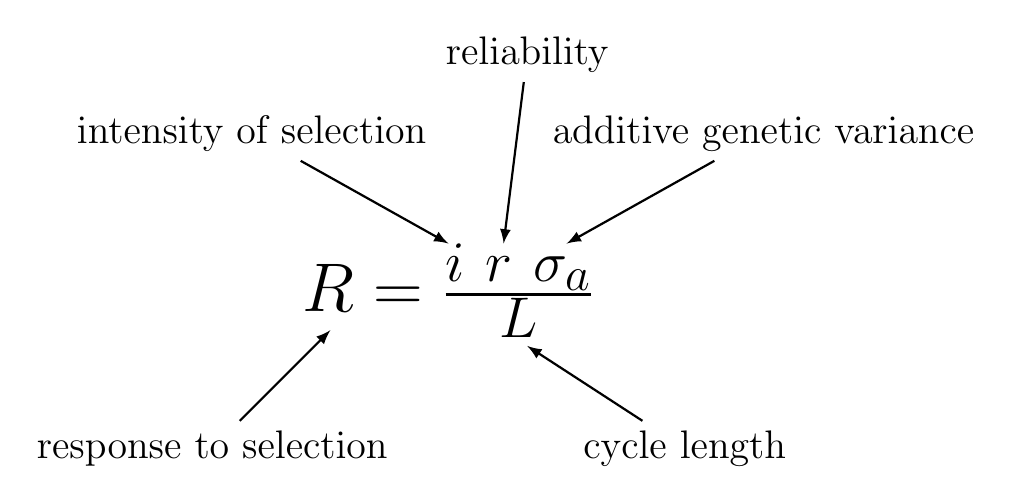
\begin{tikzpicture}
    % \node at (0, 0) {\begin{equation} R = \Delta G = \frac{ir\sigma_a}{L} \end{equation}};
    
    % \node (eq) at (0, 0) {\Huge{$R = \Delta G = \frac{i \ r \ \sigma_a}{L}$}};
    \node (eq) at (0, 0) {\Huge{$R = \frac{i \ r \ \sigma_a}{L}$}};
    
    \visible<2->{\node (R) at (-3, -2) {\Large{response to selection}};}
    \visible<2->{\draw[->, thick] (R) -- (-1.5, -0.5);}

    \visible<2->{\node (i) at (-2.5, 2) {\Large{intensity of selection}};}
    \visible<2->{\draw[->, thick] (i) -- (0, 0.6);}
    
    \visible<2->{\node (r) at (1, 3) {\Large{reliability}};}
    \visible<2->{\draw[->, thick] (r) -- (0.7, 0.6);}
    
    \visible<2->{\node (Va) at (4, 2) {\Large{additive genetic variance}};}
    \visible<2->{\draw[->, thick] (Va) -- (1.5, 0.6);}
    
    
    \visible<2->{\node (L) at (3, -2) {\Large{cycle length}};}
    \visible<2->{\draw[->, thick] (L) -- (1, -0.7);}


    \end{tikzpicture}
}

\subsection{Traditional breeding}


% \frame{\frametitle{$21^\text{st}$ Century Plant Breeding Pipeline}
\frame{\frametitle{A traditional breeding program}
% High throughput phenotypes serve \highlite{2} purposes for breeding:

\begin{columns}
\begin{column}{0.3\linewidth}
  % \highlite{How do we transition}
\highlite{Traditional Breeding}
\vspace{2mm}

  \begin{itemize}
    \item Accurate (high $r$)
    \begin{itemize}
      \item Extensive testing 
    \end{itemize}
\vspace{2mm}
\visible<6->{    
    \item Slow ()
    \begin{itemize}
      \item Multiple trial years 
      \item Long generation intervals
    \end{itemize}% \pause
  \end{itemize}
}
\vfill

\end{column}
\begin{column}{0.7\linewidth}
  % \begin{figure}[width = \linewidth]
% \vspace{-1cm}
  \begin{tikzpicture}[scale = 1]
  \begin{scope}[xshift = 0cm, yshift = 0cm, scale=0.4]
    \foreach \x in {-9, ...,9}{
    \visible<1->{\draw[draw = \plotLine, fill = \plotFill, thick, rounded corners = 0.5] (\x*0.5 - 0.1, 0) rectangle (\x*0.5 + 0.1, -2);}
    }
    \foreach \x in {-4, ...,4}{
    \visible<2->{\draw[draw = \plotLine, fill = \plotFill, thick, rounded corners = 1] (\x*0.75 - 0.25, -2.5) rectangle (\x*0.75 +0.25, -4.5);}
    }
    \foreach \x in {-2, ...,2}{
    \visible<3->{\draw[draw = \plotLine, fill = \plotFill, thick, rounded corners = 1] (\x-0.35, -5) rectangle (\x+0.35, -7);}
    }
    \foreach \x in {-1, ...,1}{
    \visible<4->{\draw[draw = \plotLine, fill = \plotFill, thick, rounded corners = 1] (\x*1.25-0.45, -7.5) rectangle (\x*1.25+0.45, -10.5);}
    }
    \node[align=left] at (0,1) {\highlite{Variety Development Pipeline}};
    \visible<1->{\node (y1) at (5,-1) {};}
    \visible<1->{\node (y2) at (4,-3.5) {};}
    \visible<1->{\node (y3) at (3,-6) {};}
    \visible<1->{\node[align=left] at (8,-1) {Year 1};}
    \visible<2->{\node[align=left] at (8,-3.5) {Year 2};}
    \visible<3->{\node[align=left] at (8,-6) {Year 3};}
    \visible<4->{\node[align=left] at (8,-9) {Year 4-5};}
    \visible<5->{\node[align=left] at (8,-12.5) {Year 6};}
    \visible<1->{\node[align=left] at (-10,-1) {$10^4$, 1 Env, unrep};}
    \visible<2->{\node[align=left] at (-10,-3.5) {$10^3$, 1 Env, low reps};}
    \visible<3->{\node[align=left] at (-10,-6) {$10^2$, few Envs, moderate reps};}
    \visible<4->{\node[align=left] at (-10,-9) {$10^1$, many Env, high reps};}
    \visible<5->{\node[align=left] at (-10,-12.5) {Variety release};}
    \end{scope}
    \begin{scope}[xshift = 0.1mm, yshift = -5cm, scale=1]
      \visible<5->{\node[label=below:``Hokie''] (pete) at (0,0) {\includegraphics[height = 1cm]{"\string~/Dropbox/wheatCartoons/aestivum"}};}
    \end{scope}
    \visible<6>{\draw [->, very thick, looseness=1.6] (pete) to [out=15, in = 330] (y1);}
    \visible<7>{\draw [->, very thick, looseness=1.6] (y3) to [out=15, in = 340] (y1);}
    \visible<7>{\node at (2, -1.5){\Large{?}};}

  \end{tikzpicture}
% \end{figure}
\end{column}


\end{columns}
}


\subsection{Breeder's equation}


\frame{
\frametitle{Which terms can we easily exploit?}
  \centering
    \begin{tikzpicture}
    % \node at (0, 0) {\begin{equation} R = \Delta G = \frac{ir\sigma_a}{L} \end{equation}};
    
    % \node (eq) at (0, 0) {\Huge{$R = \Delta G = \frac{i \ r \ \sigma_a}{L}$}};
    \node (eq) at (0, 0) {\Huge{$R = \frac{i \ r \ \sigma_a}{L}$}};
    
    \node (R) at (-3, -2) {\Large{response to selection}};
    \draw[->, thick] (R) -- (-1.5, -0.5);

    \visible<1>{\node (i) at (-2.5, 2) {\Large{intensity of selection}};}
    \draw[->, thick] (i) -- (0, 0.6);
    
    \node (r) at (1, 3) {\Large{reliability}};
    \draw[->, thick] (r) -- (0.7, 0.6);
    
    \node (Va) at (4, 2) {\Large{additive genetic variance}};
    \draw[->, thick] (Va) -- (1.5, 0.6);
    
    
    \node (L) at (3, -2) {\Large{cycle length}};
    \draw[->, thick] (L) -- (1, -0.7);

    \visible<2>{\node (i) at (-2.5, 2) {\highlite{\Large{intensity of selection}}};}
    % \visible<4->{\node (L) at (3, -2) {\highlite{\Large{cycles per year}}};}
% \visible<8>{\node (i) at (-2.5, 2) {\highlite{\Large{intensity of selection}}};}


    \end{tikzpicture}
}

\subsection{Genomic selection}
\frame{
  \frametitle{Incorporating Genomic Selection}

  \begin{columns}
  \begin{column}{0.6\linewidth}
  \begin{tikzpicture}
  
  \node at (1.5, 3) {Phenotype obs};
  \node at (4.5, 3) {Phenotype unobs};
  \node[rotate = 90] at (-1, 1.375) {DNA obs};
  \node[rotate = 90] at (-1, -1.675) {DNA unobs};

  \draw[thick] (-0.5,2.5) -- (-0.5, -3) -- (6.5, -3) -- (6.5, 2.5) --(-0.5, 2.5);
  \draw[thick] (-0.5,-0.25) -- (6.5, -0.25);
  \draw[thick] (3,2.5) -- (3, -3);


      \begin{scope}[domain=1.9:13.1, samples=101, xshift = 0cm, yshift = 0cm, scale=0.18, rotate = 60]
          \helix{\dnaA}{\dnaB}{\dnabridge}
      \end{scope}
      \begin{scope}[xshift = 2cm, yshift = 1cm, scale=1]
        \node (wheatbig) at (0,0) {\includegraphics[height = 1.6cm]{"\string~/Dropbox/wheatCartoons/aestivum"}};
      \end{scope}

    \begin{scope}[domain=1.9:13.1, samples=101, xshift = 3.5cm, yshift = 0cm, scale=0.18, rotate = 60]
          \helix{\dnaA}{\dnaB}{\dnabridge}
        \end{scope}
      \visible<1>{
      \begin{scope}[xshift = 5.5cm, yshift = 1cm, scale=1]
        \node (wheatbig) at (0,0) {\includegraphics[height = 1.6cm]{"\string~/Dropbox/wheatCartoons/aestivumDark180"}};
      \end{scope}
      }
      \visible<2->{
      \begin{scope}[xshift = 5.5cm, yshift = 1cm, scale=1]
        \node (wheatbig) at (0,0) {\includegraphics[height = 1.6cm]{"\string~/Dropbox/wheatCartoons/aestivum"}};
      \end{scope}
      }


    \begin{scope}[domain=1.9:13.1, samples=101, xshift = 0cm, yshift = -2.8cm, scale=0.18, rotate = 60]
          \helix{\graycol}{\graycol}{\graycol}
      \end{scope}
      \begin{scope}[xshift = 2cm, yshift = -1.8cm, scale=1]
        \node (wheatbig) at (0,0) {\includegraphics[height = 1.6cm]{"\string~/Dropbox/wheatCartoons/aestivum"}};
      \end{scope}

    \begin{scope}[domain=1.9:13.1, samples=101, xshift = 3.5cm, yshift = -2.8cm, scale=0.18, rotate = 60]
          \helix{\graycol}{\graycol}{\graycol}
      \end{scope}
      \begin{scope}[xshift = 5.5cm, yshift = -1.8cm, scale=1]
        \node (wheatbig) at (0,0) {\includegraphics[height = 1.6cm]{"\string~/Dropbox/wheatCartoons/aestivumDark180"}};
      \end{scope}
  \visible<2->{\draw[->, thick, Carnellian] (2.3, 1) -- (5, 1);}

  \end{tikzpicture}

  \end{column}
  \begin{column}{0.4\linewidth}
  
  Genomic prediction
  \begin{itemize}
    \item Estimate all marker effects 
    \item Predict unobserved lines based on marker scores
  \begin{itemize}
    \item \highlite{with some accuracy $< 1$}
  \end{itemize}
  \end{itemize}
  
  \vspace{3mm}
  
  \visible<3>{
  Genomic selection
  \begin{itemize}
  \item Make breeding decisions based on genomic predictions
  \begin{itemize}
    \item \highlite{increase selection intensity}
    \item \highlite{reduce cycle time}
  \end{itemize}    
  \end{itemize}
}
  \end{column}
  \end{columns}
  

}

\section{Increased selection intensity}


\subsection{Increasing population with genomic prediction}

% \frame{\frametitle{$21^\text{st}$ Century Plant Breeding Pipeline}
\frame{\frametitle{Increasing population size increases intensity}
% High throughput phenotypes serve \highlite{2} purposes for breeding:

% \begin{tikzpicture}
\begin{columns}
\begin{column}{0.4\linewidth}
\highlite{Genomic Selection}
  \begin{itemize}
    \item Less accurate
    \begin{itemize}
      \item Less phenotypic information
\visible<2->{
    \end{itemize}
    \item More intense
    \begin{itemize}
      \item Increased number of selection candidates in early trials
    \end{itemize}% \pause
}


\visible<3->{
    \item 1-2k markers $<$ \$10/line 
    \begin{itemize}
      \item Need to make up for extra costs
      \item Reduce \# of plots, less reps/line
      \item Trade for replication at a genetic level
    \end{itemize}% \pause

    % \item Faster
    % \begin{itemize}
    %   \item Short generation intervals
    % \end{itemize}% \pause
}
  \end{itemize}
% Increase number of selection candidates
% \visible<2->{
% \begin{itemize}
% \item Prediction of early performance
% \item Increased intensity in early stage trials
% \end{itemize}
% }
% \visible<3->{
% \highlite{But, genotyping will add to cost...}
% \begin{itemize}
% \item Reduce the number of yield plots 
% \item in middle stages
% \end{itemize}

\end{column}

\begin{column}{0.2\linewidth}
\centering

\begin{tikzpicture}
\begin{scope}[yshift=0cm,rotate=0]
   \node {\begin{tikzpicture}[scale = 0.3]
      \begin{axis}[%no markers, 
      ticks=none,
      domain=-3:3, 
      samples=100,
      axis x line = middle,
      x axis line style=-,
      % xticklabels=\empty,
      axis y line=none]
      \addplot [fill=white, draw=none, domain=-3:3] {gauss(0,1)} \closedcycle;
      \addplot [fill=black, draw=none, domain=0.524:3] {gauss(0,1)} \closedcycle;
      \addplot[black] {gauss(0,1)};
      \end{axis}
    \end{tikzpicture}};

   \visible<2->{\node at (0, -2) {\begin{tikzpicture}[scale = 0.6, yscale = 0.5]
      \begin{axis}[%no markers, 
      ticks=none,
      domain=-6:6, 
      samples=100,
      axis x line = middle,
      x axis line style=-,
      % xticklabels=\empty,
      axis y line=none]
      \addplot [fill=white, draw=none, domain=-6:6] {gauss(0,2)} \closedcycle;
      \addplot [fill=black, draw=none, domain=2.07:6] {gauss(0,2)} \closedcycle;
      \addplot[black] {gauss(0,2)};
      \end{axis}
    \end{tikzpicture}};
\draw[Carnellian] (0,0.7) -- (0, -2.7);
}
\end{scope}

\end{tikzpicture}
\end{column}

\begin{column}{0.4\linewidth}
  % \begin{figure}[width = \linewidth]
% \vspace{-1cm}
  \begin{tikzpicture}[scale = 1]
  \begin{scope}[xshift = 0cm, yshift = 0cm, scale=0.4]
    \foreach \x in {-14, ...,10}{
    \visible<2->{\draw[draw = \graycol, fill = \graycol, thick, rounded corners = 0.5] (\x*0.5 - 0.1, 0) rectangle (\x*0.5 + 0.1, -2);}
    }
    \foreach \x in {-10, ...,14}{
    \visible<2->{\draw[draw = \graycol, fill = \graycol, thick, rounded corners = 0.5] (\x*0.5 - 0.1, 0) rectangle (\x*0.5 + 0.1, -2);}
    }

    \foreach \x in {-7, -6, -5, 5, 6, 7}{
    \visible<2->{\draw[draw = \graycol, fill = \graycol, thick, rounded corners = 1] (\x*0.75 - 0.25, -2.5) rectangle (\x*0.75 +0.25, -4.5);}
    }
    \foreach \x in {-3,3}{
    \visible<2->{\draw[draw = \graycol, fill = \graycol, thick, rounded corners = 1] (\x-0.35, -5) rectangle (\x+0.35, -7);}
    }


    \foreach \x in {-9, ...,9}{
    \draw[draw = \plotLine, fill = \plotFill, thick, rounded corners = 0.5] (\x*0.5 - 0.1, 0) rectangle (\x*0.5 + 0.1, -2);
    }
    \foreach \x in {-4, ...,4}{
    \draw[draw = \plotLine, fill = \plotFill, thick, rounded corners = 1] (\x*0.75 - 0.25, -2.5) rectangle (\x*0.75 +0.25, -4.5);
    }
    \foreach \x in {-2, ...,2}{
    \draw[draw = \plotLine, fill = \plotFill, thick, rounded corners = 1] (\x-0.35, -5) rectangle (\x+0.35, -7);
    }
    \foreach \x in {-1, ...,1}{
    \draw[draw = \plotLine, fill = \plotFill, thick, rounded corners = 1] (\x*1.25-0.45, -7.5) rectangle (\x*1.25+0.45, -10.5);
    }
    \draw[draw = \plotLine, fill = \plotFill, thick, rounded corners = 1] (-0.45, -11) rectangle (0.45, -14);
    \node[align=left] at (0,1) {\highlite{Variety Development Pipeline}};
    \visible<1->{\node (y1) at (5,-1) {};}
    \end{scope}
    % \fill[bottom color=Carnellian, top color=Carnellian!50!white, anchor=south] (3.5, 0) -- (3.5, -5.5) --(2, -5.5) --(3.5, 0);
    % \node[LightGray] at (3, -5) {$h^2$};
]
  \end{tikzpicture}
% \end{figure}
\end{column}

\end{columns}
}

\subsection{Unobserved vs sparse testing prediction}

\frame{\frametitle{Current model for genomic prediction works...}
  \begin{columns}
 
  \begin{column}{0.3\linewidth}
  
  % Two Environments
  \begin{enumerate}
    \item Observe half of population in both environments
    \item Estimate genetic correlation of environments
    \item Predict other half
  \end{enumerate}
  \end{column}


  \begin{column}{0.3\linewidth}
  \begin{tikzpicture}[scale = 0.7, auto,node distance=1cm,very thick]
 

\draw[thick, draw=Navy] (0,0) rectangle(2, 4);
\draw[thick, draw=Navy, fill=Navy] (0,2) rectangle(2, 4);
\draw[thick, draw=Navy] (2.5,0) rectangle(4.5, 4);
\draw[thick, draw=Navy, fill=Navy] (2.5,2) rectangle(4.5, 4);
% \draw[thick, draw, fill=black] (0,1) rectangle(2, 2);

\draw[->, draw=Carnellian] (1,3) to (1, 1.2);
\draw[->, draw=Carnellian] (1,3) to (3.3, 1.2);
% \draw[->, draw=Carnellian] (1,3) to (3.5, 1);
\draw[->, draw=Carnellian] (3.5,3) to (1.2, 1.2);
\draw[->, draw=Carnellian] (3.5,3) to (3.5, 1.2);

% \begin{scope}[yshift=0cm,xshift=6cm,rotate=0]
% \draw[thick, draw=Navy] (0,0) rectangle(2, 4);
% \draw[thick, draw=Navy, fill=Navy] (0,2) rectangle(2, 4);
% \draw[thick, draw=Navy] (2.5,0) rectangle(4.5, 4);
% \draw[thick, draw=Navy, fill=Navy] (2.5,0) rectangle(4.5, 2);

% \draw[->, draw=Carnellian] (1,3) to (3.3, 3);
% \draw[->, draw=Carnellian] (1,3) to (1, 1.2);
% % \draw[->, draw=Carnellian] (1,3) to (3.5, 1);
% \draw[->, draw=Carnellian] (3.5,1) to (1.2, 1);
% \draw[->, draw=Carnellian] (3.5,1) to (3.5, 2.8);


% \end{scope}


\node[align=center, rotate=90] (g) at (-1, 2) {\highlite{Genotypes}};
\node[align=center] (env) at (2.5, 5.5) {\highlite{Environments}};

\node[align=center] (irr) at (1, 4.5) {Optimal};
\node[align=center] (rain) at (3.5, 4.5) {Drought};
% \node[align=center] (chickpea) at (2.25, -0.5) {Chickpea};
% \node[align=center] (e1) at (7, 4.5) {Optimal};
% \node[align=center] (e2) at (9.5, 4.5) {Drought};

\node[align=center] (e1) at (2.5, -1) {Unobserved / Full-sib \\ prediction};
% \node[align=center] (e2) at (8, -1) {Sparse Testing};

\begin{scope}[yshift=7cm,xshift=0.5cm,rotate=0]
\node[thick, draw=Navy, fill=Navy, text = LightGray] (obs) at (0,0) {observed};
\node[thick, draw=Navy, text = DarkGray] (unobs) at (3,0) {predicted};
\end{scope}

% \node[align=center] (maize) at (8.5, -0.5) {Maize};

\end{tikzpicture}

  \end{column}


\pause
  \begin{column}{0.4\linewidth}
\centering
  
  \includegraphics[width= \linewidth]{"\string ~/Dropbox/plantGenomicsCongress/cimmytMaizeAcc"} \\
  Beyene et al. 2020
  \end{column}

  \end{columns}

}


\frame{\frametitle{... but can we do better?}

\begin{columns}
\begin{column}{0.4\linewidth}
  Genetic relationships known
  \begin{itemize}
    \item estimate genetic correlation of environments without replicating across 
    \item Get to observe every line
  \end{itemize}
\end{column}
\begin{column}{0.6\linewidth}
\centering
% \visible<3>{
\begin{tikzpicture}[scale = 0.7, auto,node distance=1cm,very thick]
 
\begin{scope}[yshift=7cm,xshift=4cm,rotate=0]
\node[thick, draw=Navy, fill=Navy, text = LightGray] (obs) at (0,0) {observed};
\node[thick, draw=Navy, text = DarkGray] (unobs) at (3,0) {predicted};
\end{scope}

\draw[thick, draw=Navy] (0,0) rectangle(2, 4);
\draw[thick, draw=Navy, fill=Navy] (0,2) rectangle(2, 4);
\draw[thick, draw=Navy] (2.5,0) rectangle(4.5, 4);
\draw[thick, draw=Navy, fill=Navy] (2.5,2) rectangle(4.5, 4);
% \draw[thick, draw, fill=black] (0,1) rectangle(2, 2);

\draw[->, draw=Carnellian] (1,3) to (1, 1.2);
\draw[->, draw=Carnellian] (1,3) to (3.3, 1.2);
% \draw[->, draw=Carnellian] (1,3) to (3.5, 1);
\draw[->, draw=Carnellian] (3.5,3) to (1.2, 1.2);
\draw[->, draw=Carnellian] (3.5,3) to (3.5, 1.2);

\node[align=center, rotate=90] (g) at (-1, 2) {\highlite{Genotypes}};
\node[align=center] (env) at (5.5, 5.5) {\highlite{Environments}};

\node[align=center] (irr) at (1, 4.5) {Optimal};
\node[align=center] (rain) at (3.5, 4.5) {Drought};
% \node[align=center] (chickpea) at (2.25, -0.5) {Chickpea};

\node[align=center] (e1) at (2.5, -1) {Unobserved / Full-sib \\ prediction};

\visible<2>{
  
\begin{scope}[yshift=0cm,xshift=6cm,rotate=0]
\draw[thick, draw=Navy] (0,0) rectangle(2, 4);
\draw[thick, draw=Navy, fill=Navy] (0,2) rectangle(2, 4);
\draw[thick, draw=Navy] (2.5,0) rectangle(4.5, 4);
\draw[thick, draw=Navy, fill=Navy] (2.5,0) rectangle(4.5, 2);

\draw[->, draw=Carnellian] (1,3) to (3.3, 3);
\draw[->, draw=Carnellian] (1,3) to (1, 1.2);
% \draw[->, draw=Carnellian] (1,3) to (3.5, 1);
\draw[->, draw=Carnellian] (3.5,1) to (1.2, 1);
\draw[->, draw=Carnellian] (3.5,1) to (3.5, 2.8);

\end{scope}


\node[align=center] (e1) at (7, 4.5) {Optimal};
\node[align=center] (e2) at (9.5, 4.5) {Drought};
\node[align=center] (e2) at (8, -1) {Sparse Testing};
% }
% \node[align=center] (maize) at (8.5, -0.5) {Maize};

}
\end{tikzpicture}
\end{column}
\end{columns}

}


% \subsection{Sparse testing vs unobserved prediction}

\frame{\frametitle{Sparse testing is (almost) uniformly superior to unobserved prediction}

% \vspace{-0.2cm}

% \hspace{2.5cm} CIMMYT Maize \hspace{5cm} \visible<2>{ICRISAT Chickpea}

\vspace{-0.5cm}

\begin{tikzpicture}
\node at (0, 0) {\includegraphics[width= 0.5\linewidth]{"\string /home/nsant/Dropbox/sparseTesting/sparseVsHalfMaizePres"}};
\node at (8, 0) {\includegraphics[width= 0.5\linewidth]{"\string /home/nsant/Dropbox/chickpeaGit/figures/sparseVsHalfChickpeaPres"}};

\node at (0, 3.2) {CIMMYT Maize};
\node at (8, 3.2) {ICRISAT Chickpea};

\begin{scope}[yshift=2.2cm,xshift=1.2cm,scale=0.15]
\draw[thick, draw=Navy] (0,0) rectangle(2, 4);
\draw[thick, draw=Navy, fill=Navy] (0,2) rectangle(2, 4);
\draw[thick, draw=Navy] (2.5,0) rectangle(4.5, 4);
\draw[thick, draw=Navy, fill=Navy] (2.5,0) rectangle(4.5, 2);
\end{scope}

\begin{scope}[yshift=1cm,xshift=2cm,scale=0.15]
\draw[thick, draw=Navy] (0,0) rectangle(2, 4);
\draw[thick, draw=Navy, fill=Navy] (0,2) rectangle(2, 4);
\draw[thick, draw=Navy] (2.5,0) rectangle(4.5, 4);
\draw[thick, draw=Navy, fill=Navy] (2.5,2) rectangle(4.5, 4);
\end{scope}


% \visible<2>{
\begin{scope}[yshift=2.2cm,xshift=9.2cm,scale=0.15]
\draw[thick, draw=Navy] (0,0) rectangle(2, 4);
\draw[thick, draw=Navy, fill=Navy] (0,2) rectangle(2, 4);
\draw[thick, draw=Navy] (2.5,0) rectangle(4.5, 4);
\draw[thick, draw=Navy, fill=Navy] (2.5,0) rectangle(4.5, 2);
\end{scope}

\begin{scope}[yshift=1cm,xshift=10cm,scale=0.15]
\draw[thick, draw=Navy] (0,0) rectangle(2, 4);
\draw[thick, draw=Navy, fill=Navy] (0,2) rectangle(2, 4);
\draw[thick, draw=Navy] (2.5,0) rectangle(4.5, 4);
\draw[thick, draw=Navy, fill=Navy] (2.5,2) rectangle(4.5, 4);
\end{scope}
% }

\end{tikzpicture}

}

\subsection{Using HTP to recover genotyping costs}

\frame{
  \frametitle{Marginal savings from plot reduction}
\begin{columns}
\begin{column}{0.5\linewidth}
Still have to...
  \begin{itemize}
    \item Plant all locations 
    \item Take notes all locations
    \item Harvest all locations
  \end{itemize}

\vspace{3mm}

\visible<2->{
Use drone in place of a note taker or harvester?
  \begin{itemize}
    \item All plots imaged
    \item Only some plots harvested
    \item Use multi-trait models
  \end{itemize}
}
\end{column}

\begin{column}{0.5\linewidth}
\centering
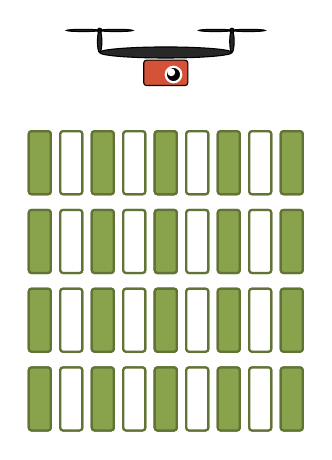
\begin{tikzpicture}[scale = 1]
  \visible<2->{
  \begin{scope}[xshift = 0cm, yshift = 1cm, scale=0.14]
      \drone{\dronedrawcol}{\dronefillcol}{\dronebladecol}{\dronecameracol}
  \end{scope}
  }
  \visible<1-2>{
  \begin{scope}[xshift = 0cm, yshift = 0cm, scale=0.4]
    \foreach \x in {-4, ...,4}{
      \draw[draw = \plotLine, fill = \plotFill, thick, rounded corners = 1] (\x-0.35, 0) rectangle (\x+0.35, -2);
    }
    \foreach \x in {-4, ...,4}{
      \draw[draw = \plotLine, fill = \plotFill, thick, rounded corners = 1] (\x-0.35, -2.5) rectangle (\x+0.35, -4.5);
    }
    \foreach \x in {-4, ...,4}{
      \draw[draw = \plotLine, fill = \plotFill, thick, rounded corners = 1] (\x-0.35, -5) rectangle (\x+0.35, -7);
    }

    \foreach \x in {-4, ...,4}{
      \draw[draw = \plotLine, fill = \plotFill, thick, rounded corners = 1] (\x-0.35, -7.5) rectangle (\x+0.35, -9.5);
    }

    \end{scope}
    }

  \visible<3->{
  \begin{scope}[xshift = 0cm, yshift = 0cm, scale=0.4]
    \foreach \x in {-4, -2, 0, 2, ,4}{
      \draw[draw = \plotLine, fill = \plotFill, thick, rounded corners = 1] (\x-0.35, 0) rectangle (\x+0.35, -2);
    }

    \foreach \x in {-3, -1, 1, 3}{
      \draw[draw = \plotLine, fill = white, thick, rounded corners = 1] (\x-0.35, 0) rectangle (\x+0.35, -2);
    }

    \foreach \x in {-4, -2, 0, 2, ,4}{
      \draw[draw = \plotLine, fill = \plotFill, thick, rounded corners = 1] (\x-0.35, -2.5) rectangle (\x+0.35, -4.5);
    }

    \foreach \x in {-3, -1, 1, 3}{
      \draw[draw = \plotLine, fill = white, thick, rounded corners = 1] (\x-0.35, -2.5) rectangle (\x+0.35, -4.5);
    }
    \foreach \x in {-4, -2, 0, 2, ,4}{
      \draw[draw = \plotLine, fill = \plotFill, thick, rounded corners = 1] (\x-0.35, -5) rectangle (\x+0.35, -7);
    }

    \foreach \x in {-3, -1, 1, 3}{
      \draw[draw = \plotLine, fill = white, thick, rounded corners = 1] (\x-0.35, -5) rectangle (\x+0.35, -7);
    }

    \foreach \x in {-4, -2, 0, 2, ,4}{
      \draw[draw = \plotLine, fill = \plotFill, thick, rounded corners = 1] (\x-0.35, -7.5) rectangle (\x+0.35, -9.5);
    }

    \foreach \x in {-3, -1, 1, 3}{
      \draw[draw = \plotLine, fill = white, thick, rounded corners = 1] (\x-0.35, -7.5) rectangle (\x+0.35, -9.5);
    }

    \end{scope}
    }
    % \fill[bottom color=Carnellian, top color=Carnellian!50!white, anchor=south] (3.5, 0) -- (3.5, -5.5) --(2, -5.5) --(3.5, 0);
    % \node[LightGray] at (3, -5) {$h^2$};
]
  \end{tikzpicture}
  \end{column}
  \end{columns}
}


\frame{
  \frametitle{Use HTPs to correct for spatial variability, increase intensity}

  \begin{columns}
  \begin{column}{0.6\linewidth}
  \centering
    \begin{tikzpicture}
      \node (y) at (0, 3.7) {\includegraphics[width=3cm]{"\string~/Dropbox/interviewFigs/AR1y"}};
      \node (g) at (-2, 0) {\includegraphics[width=3cm]{"\string~/Dropbox/interviewFigs/AR1g"}};
      \node (e) at (2, 0) {\includegraphics[width=3cm]{"\string~/Dropbox/interviewFigs/AR1e"}};
      \draw[->, DarkGray] (y) -- (g);
      \draw[->, DarkGray] (y) -- (e);
    \end{tikzpicture}
  \end{column}
  \begin{column}{0.4\linewidth}
    
    % High throughput phenotypes are cheap!
    High throughput phenotypes
    \begin{itemize}
      \item Track genetic \& spatial variation 
      \item Monitor growth, disease progression (scab?)
    \end{itemize}
  \vspace{5mm}
    Can use to.
    \begin{itemize}
      \item Reduce replication
      \item Increase entries (i.e. increase $i$)
      \item \highlite{Reduce time to Multi-Env. Trials}
    \end{itemize}

    Potential SmartFarm Collaboration?

  \end{column}
  \end{columns}

}

% \frame{
%   \frametitle{}
% }


\subsection{Genotype specific growth curves}
\frame{
 \frametitle{Use imagery to model growth, predict G$\times$E}
 \begin{animateinline}[controls, autoplay,loop]{2}
 % \begin{animateinline}[autoplay,loop]{2}
   % \multiframe{21}{i=1+1}{
   \multiframe{21}{i=1+1}{
     \begin{tikzpicture}
       \node[inner sep=0pt] at (0,0) {\includegraphics[width=0.5\textwidth]{../../alfalfaGeneva/animateOrtho/ortho\i}};
       \node[inner sep=0pt] at (8,0) {\includegraphics[width=0.5\textwidth]{../../interviewFigs/egGrowthCurvesAnimatePNGs/pg-\i}};
      % \node at (0, 0) {\animategraphics[controls, width = 0.6\linewidth]{1}{../../alfalfaGeneva/animateOrtho/ortho}{1}{21}};
    \draw[thick, optiyellow] (-1.8, -0.07) rectangle (-0.7, 0.18);
    \draw[thick, optipurple] (-1.8, 0.75) rectangle (-0.7, 1);
    \draw[thick, optiblue] (-1.8, -0.65) rectangle (-0.7, -0.9);
     \end{tikzpicture}
   }
 \end{animateinline}
}




\frame{
\frametitle{Time is on our side}
  \centering
    \begin{tikzpicture}
    % \node at (0, 0) {\begin{equation} R = \Delta G = \frac{ir\sigma_a}{L} \end{equation}};
    
    % \node (eq) at (0, 0) {\Huge{$R = \Delta G = \frac{i \ r \ \sigma_a}{L}$}};
    \node (eq) at (0, 0) {\Huge{$R = \frac{i \ r \ \sigma_a}{L}$}};
    
    \node (R) at (-3, -2) {\Large{response to selection}};
    \draw[->, thick] (R) -- (-1.5, -0.5);

    \node (i) at (-2.5, 2) {\Large{intensity of selection}};
    \draw[->, thick] (i) -- (0, 0.6);
    
    \node (r) at (1, 3) {\Large{reliability}};
    \draw[->, thick] (r) -- (0.7, 0.6);
    
    \node (Va) at (4, 2) {\Large{additive genetic variance}};
    \draw[->, thick] (Va) -- (1.5, 0.6);
    
    
    \node (L) at (3, -2) {\Large{cycle length}};
    \draw[->, thick] (L) -- (1, -0.7);


    % \visible<3->{\node (i) at (-2.5, 2) {\highlite{\Large{intensity of selection}}};}
    \visible<2->{\node (L) at (3, -2) {\highlite{\Large{cycle length}}};}
% \visible<8>{\node (i) at (-2.5, 2) {\highlite{\Large{intensity of selection}}};}


    \end{tikzpicture}
}



\section{Rapid cycling}
\subsection{In theory}

% \frame{\frametitle{$21^\text{st}$ Century Plant Breeding Pipeline}
\frame{\frametitle{Rapid cycling greatly decreases $L$}
% High throughput phenotypes serve \highlite{2} purposes for breeding:

\begin{columns}
\begin{column}{0.3\linewidth}
  % \highlite{How do we transition}
\highlite{Rapid Cycling}
\begin{itemize}
  \item Assume 3 cycles/year in greenhouse
\end{itemize}

\centering

\begin{tikzpicture}
    % \node (rcrs) at (0, 0) {\begin{tabular}{c} Recurrent\\Pop \end{tabular}};
   \node (rcrs) at (0, 0) {\begin{tikzpicture}[scale = 0.2]
      \begin{axis}[%no markers, 
      ticks=none,
      domain=-3:3, 
      samples=100,
      axis x line = middle,
      x axis line style=-,
      % xticklabels=\empty,
      axis y line=none]
      \addplot [fill=white, draw=none, domain=-3:3] {gauss(0,1)} \closedcycle;
      \addplot [fill=dgray, draw=none, domain=0.524:3] {gauss(0,1)} \closedcycle;
      \addplot[dgray] {gauss(0,1)};
      \end{axis}
    \end{tikzpicture}};

    \visible<2->{\draw [->,dgray, very thick] ([shift=(445:1cm)] 0,0) arc (445:335:1cm);}
    \visible<3->{\draw [->,dgray, very thick] ([shift=(325:1cm)] 0,0) arc (325:215:1cm);}
    \visible<4->{\draw [->,dgray, very thick] ([shift=(205:1cm)] 0,0) arc (205:95:1cm);}
    \visible<5->{\draw [->,dgray, very thick] ([shift=(445:1.25cm)] 0,0) arc (445:335:1.25cm);}
    \visible<6->{\draw [->,dgray, very thick] ([shift=(325:1.25cm)] 0,0) arc (325:215:1.25cm);}
    \visible<7->{\draw [->,dgray, very thick] ([shift=(205:1.25cm)] 0,0) arc (205:95:1.25cm);}
    \visible<8->{\draw [->,dgray, very thick] ([shift=(445:1.5cm)] 0,0) arc (445:335:1.5cm);}
    \visible<9->{\draw [->,dgray, very thick] ([shift=(325:1.5cm)] 0,0) arc (325:215:1.5cm);}
    \visible<10->{\draw [->,dgray, very thick] ([shift=(205:1.5cm)] 0,0) arc (205:95:1.5cm);}
    \visible<11->{\draw [->,dgray, very thick] ([shift=(445:1.75cm)] 0,0) arc (445:335:1.75cm);}
    \visible<12->{\draw [->,dgray, very thick] ([shift=(325:1.75cm)] 0,0) arc (325:215:1.75cm);}
    \visible<13->{\draw [->,dgray, very thick] ([shift=(205:1.75cm)] 0,0) arc (205:95:1.75cm);}
\end{tikzpicture}


\end{column}
\begin{column}{0.4\linewidth}
  % \begin{figure}[width = \linewidth]
% \vspace{-1cm}
  \begin{tikzpicture}[scale = 1]
  \begin{scope}[xshift = 0cm, yshift = 0cm, scale=0.3]
    \foreach \x in {-9, ...,9}{
    \visible<1->{\draw[draw = \plotLine, fill = \plotFill, thick, rounded corners = 0.5] (\x*0.5 - 0.1, 0) rectangle (\x*0.5 + 0.1, -2);}
    }
    \foreach \x in {-4, ...,4}{
    \visible<4->{\draw[draw = \plotLine, fill = \plotFill, thick, rounded corners = 1] (\x*0.75 - 0.25, -2.5) rectangle (\x*0.75 +0.25, -4.5);}
    }
    \foreach \x in {-2, ...,2}{
    \visible<7->{\draw[draw = \plotLine, fill = \plotFill, thick, rounded corners = 1] (\x-0.35, -5) rectangle (\x+0.35, -7);}
    }
    \foreach \x in {-1, ...,1}{
    \visible<10->{\draw[draw = \plotLine, fill = \plotFill, thick, rounded corners = 1] (\x*1.25-0.45, -7.5) rectangle (\x*1.25+0.45, -10.5);}
    }
    \visible<13->{\draw[draw = \plotLine, fill = \plotFill, thick, rounded corners = 1] (-0.45, -11) rectangle (0.45, -14);}
    \node[align=left] at (0,1) {\highlite{Variety Development Pipeline}};
    \node (y1) at (5,-1) {};
    \node (y2) at (4,-3.5) {};
    \node (y3) at (3,-6) {};
    \visible<1->{\node[align=left] at (7,-1) {Year 1};}
    \visible<4->{\node[align=left] at (7,-3.5) {Year 2};}
    \visible<7->{\node[align=left] at (7,-6) {Year 3};}
    \visible<10->{\node[align=left] at (7,-9) {Year 4};}
    \visible<13->{\node[align=left] at (7,-12.5) {Year 5};}
    \end{scope}
    % \begin{scope}[xshift = 0.1mm, yshift = -5cm, scale=1]
    %   \visible<5->{\node[label=below:``Pistol Pete''] (pete) at (0,0) {\includegraphics[height = 1cm]{"\string~/Dropbox/wheatCartoons/aestivum"}};}
    % \end{scope}
    \visible<14->{\draw [->, very thick, looseness=1.6] (0.3, -3.8) to [out=15, in = 330] (y1);}
    % \visible<10>{\draw [->, very thick, looseness=1.6] (y3) to [out=15, in = 340] (y1);}

  \end{tikzpicture}
% \end{figure}
\end{column}

\begin{column}{0.3\linewidth}
  \includegraphics<2>[page = 1, width = 0.9\linewidth]{"\string~/Dropbox/interviewFigs/GSvsPS_1cyc"}%
  \includegraphics<3>[page = 2, width = 0.9\linewidth]{"\string~/Dropbox/interviewFigs/GSvsPS_1cyc"}%
  \includegraphics<4>[page = 3, width = 0.9\linewidth]{"\string~/Dropbox/interviewFigs/GSvsPS_1cyc"}%
  \includegraphics<5>[page = 4, width = 0.9\linewidth]{"\string~/Dropbox/interviewFigs/GSvsPS_1cyc"}%
  \includegraphics<6>[page = 5, width = 0.9\linewidth]{"\string~/Dropbox/interviewFigs/GSvsPS_1cyc"}%
  \includegraphics<7>[page = 6, width = 0.9\linewidth]{"\string~/Dropbox/interviewFigs/GSvsPS_1cyc"}%
  \includegraphics<8>[page = 7, width = 0.9\linewidth]{"\string~/Dropbox/interviewFigs/GSvsPS_1cyc"}%
  \includegraphics<9>[page = 8, width = 0.9\linewidth]{"\string~/Dropbox/interviewFigs/GSvsPS_1cyc"}%
  \includegraphics<10>[page = 9, width = 0.9\linewidth]{"\string~/Dropbox/interviewFigs/GSvsPS_1cyc"}%
  \includegraphics<11>[page = 10, width = 0.9\linewidth]{"\string~/Dropbox/interviewFigs/GSvsPS_1cyc"}%
  \includegraphics<12>[page = 11, width = 0.9\linewidth]{"\string~/Dropbox/interviewFigs/GSvsPS_1cyc"}%
  \includegraphics<13>[page = 12, width = 0.9\linewidth]{"\string~/Dropbox/interviewFigs/GSvsPS_1cyc"}%
  \includegraphics<14>[page = 13, width = 0.9\linewidth]{"\string~/Dropbox/interviewFigs/GSvsPS_1cyc"}%
\includegraphics<15>[page = 37, width = 0.9\linewidth]{"\string~/Dropbox/interviewFigs/GSvsPS_3cyc"}%
\end{column}
\end{columns}
}


\section{Rapid cycling}

\subsection{Rapid cycle recurrent truncation selection} 

\frame{\frametitle{Rapid cycle recurrent truncation beats traditional, at first}
\begin{columns}
\begin{column}{0.02\linewidth}
\end{column}
\begin{column}{0.45\linewidth}
  \includegraphics[width= 0.9\linewidth]{{{"\string /home/nsant/Dropbox/VDPfig/truncation"}}}%
\end{column}
\begin{column}{0.45\linewidth}
  \visible<2>{\includegraphics[width= 0.85\linewidth]{{{"\string /home/nsant/Dropbox/optiBreedSim/figsForPres/forKellyPresIowa/truncation20x75"}}}}%
\begin{column}{0.02\linewidth}
\end{column}

%   \visible<1-2>{Recurrent truncation selection using GEBVs in recurrent population. 
%     \begin{enumerate}
%       \item Randomly mate best predicted individuals in recurrent population
%       \item 3 cycles per year
%       \item Update genomic prediction models with phenotypes from VDP
%       \item DH $f$ best heterozygous lines in recurrent population to form $n$ lines per family $\rightarrow$ VDP
%       \item Rinse and repeat
%     \end{enumerate}
% }
\end{column}
\end{columns}
}

\subsection{Optimal contribution} 

\frame{\frametitle{Parent selection must balance mean and variance}
\vspace{-1cm}
  \begin{columns}
    \begin{column}{0.5\linewidth}
      \centering
      % \includegraphics<1-2>[width = \linewidth, page = 3]{{{"\string ~/Dropbox/PAG2019/increaseMean"}}}%
      \includegraphics<1-2>[height = 8cm, page = 3]{{{"\string ~/Dropbox/PAG2019/increaseMean"}}}%
    \end{column}
    \begin{column}{0.5\linewidth}
      \centering
      % \includegraphics<2>[height = \linewidth, page = 3, clip, trim = 0.7cm 0cm 0cm 0cm]{{{"\string ~/Dropbox/PAG2019/increaseVar"}}}%
      \includegraphics<2>[height = 8cm, page = 3, clip, trim = 0.7cm 0cm 0cm 0cm]{{{"\string ~/Dropbox/PAG2019/increaseVar"}}}%
    \end{column}
  \end{columns}
}

% \subsection{Optimal contribution} 

% \frame{\frametitle{Optimal Contribution (OC): Balance genetic gain and inbreeding}
% % From Akdemir et al. (2019):
% \begin{columns}
% \begin{column}{0.6\linewidth}
% \begin{itemize}
%   \item Let $\mathbf{b} = $ vector of GEBVs, $\text{E}[\mathbf{b}] = 0$
%   \item Let Var$(\mathbf{b}) = \sigma^2_a \mathbf{K}$
%   \item Let $\mathbf{c} = $ vector of proportional parent contributions, s.t.
%     \begin{itemize}
%       \item $\mathbf{c}'\mathbf{1} = 1$
%       \item $\mathbf{c} \geq 0$
%     \end{itemize}
% \end{itemize}
% % \pause
%   \vspace{5mm}
%   Expected gain: $\Delta_g = \mathbf{c}'\mathbf{b}$

%   \vspace{5mm}
%   Change in inbreeding: $\Delta_f = \mathbf{c}'\mathbf{K}\mathbf{c}$
% % \pause

%   \vspace{5mm}
%   For some $\lambda$, 
%   minimize $Q(\mathbf{c}) = \lambda \mathbf{c}'\mathbf{K}\mathbf{c} - (1-\lambda) \mathbf{c}'\mathbf{b}$. $\rightarrow$ Quadratic programmming
% % \pause

% \end{column}
% \begin{column}{0.4\linewidth}

%   % \vspace{5mm}
%   % How to choose $\lambda$?

%   \includegraphics<2>[width = \linewidth]{{{"\string~/Dropbox/optiBreedSim/figures/qp"}}}
% \end{column}
% \end{columns}

% }

\frame{\frametitle{Optimal contributions of parents}
% From Akdemir et al. (2019):


\begin{columns}
\begin{column}{0.5\linewidth}
Balance genetic gain and inbreeding
    \begin{itemize}
      \item Minimize inbreeding given desired gain
      \item Maximize gain given acceptable inbreeding
      \item See Meuwissen, 1997
    \end{itemize}
\vspace{3mm}
Portfolio optimization problem 
    \begin{itemize}
      \item Solve with quadratic programming 
      % \item Produce a Pareto frontier
    \item \highlite{Doesn't always pick the ``best'' individuals}
    \item \highlite{Parental contributions vary}
    \end{itemize}
\end{column}
\begin{column}{0.5\linewidth}
\visible<2>{
\begin{tikzpicture}
\node at (0, 0) {\includegraphics<2>[width = 0.85\linewidth, clip, trim = 1cm 1cm 1cm 1cm]{"\string~/Dropbox/optiBreedSim/figures/qp"}};%
\node at (0, -3.5) {$\Delta$ Gain};%
\node[rotate=90] at (-3.6, 0) {$\Delta$ Inbreeding};%
\end{tikzpicture}
}
\end{column}
\end{columns}

}

% \subsection{Optimal contributions} 

\frame{\frametitle{Optimal contributions can maintain $V_g$ at the cost of short-term gains}
\begin{columns}
\begin{column}{0.05\linewidth}
\end{column}
\begin{column}{0.45\linewidth}
  \includegraphics<1>[width= \linewidth]{{{"\string /home/nsant/Dropbox/VDPfig/optiCont"}}}%
  % \includegraphics<2->[width= \linewidth]{{{"\string /home/nsant/Dropbox/VDPfig/optiContBranchWithPheno"}}}%
\end{column}
\begin{column}{0.45\linewidth}
  \includegraphics<1>[width= \linewidth, page = 1]{{{"\string /home/nsant/Dropbox/optiBreedSim/figures/bestModels20x75/bestNoOCBorOCBpR"}}}%
  % \includegraphics<2>[width= \linewidth, page = 1]{{{"\string /home/nsant/Dropbox/optiBreedSim/figures/bestModels20x75/bestNoOCB"}}}%
  % \includegraphics<3>[width= \linewidth, page = 8]{{{"\string /home/nsant/Dropbox/optiBreedSim/figures/bestModels20x75/bestRTvsOCBpR"}}}%

  % \includegraphics<8>[width= 0.5\linewidth, page = 6]{{{"\string /home/nsant/Dropbox/optiBreedSim/figsForPres/optiContBranchPhenoRGSC20x75"}}}%
\end{column}
\begin{column}{0.05\linewidth}
\end{column}
\end{columns}

}


\subsection{Optimal contribution with branching} 

\frame{\frametitle{Can we have our cake and eat it too?}
\begin{columns}
\begin{column}{0.05\linewidth}
\end{column}
\begin{column}{0.45\linewidth}
  % \includegraphics<1>[width= \linewidth]{{{"\string /home/nsant/Dropbox/VDPfig/optiCont"}}}%
  \includegraphics<1->[width= \linewidth]{{{"\string /home/nsant/Dropbox/VDPfig/optiContBranchWithPheno"}}}%
\end{column}
\begin{column}{0.45\linewidth}
  % \includegraphics<1>[width= \linewidth, page = 1]{{{"\string /home/nsant/Dropbox/optiBreedSim/figures/bestModels20x75/bestNoOCBorOCBpR"}}}%
  \includegraphics<1>[width= \linewidth, page = 1]{{{"\string /home/nsant/Dropbox/optiBreedSim/figures/bestModels20x75/bestNoOCB"}}}%
  \includegraphics<2>[width= \linewidth, page = 8]{{{"\string /home/nsant/Dropbox/optiBreedSim/figures/bestModels20x75/bestRTvsOCBpR"}}}%

  % \includegraphics<8>[width= 0.5\linewidth, page = 6]{{{"\string /home/nsant/Dropbox/optiBreedSim/figsForPres/optiContBranchPhenoRGSC20x75"}}}%
\end{column}
\begin{column}{0.05\linewidth}
\end{column}
\end{columns}
}

\subsection{Conclusions from simulations}

\frame{\frametitle{Rapid cycling }
  
  % Genomic information can be used to
  % Genetic means and variances 
  % \begin{itemize}
  %   \item Truncation 
  %   \item link seemingly unrelated trials
  % \end{itemize}
\begin{columns}
\begin{column}{0.7\linewidth}
% Truncation
%   \begin{itemize}
%     \item Short-term gains 
%     \item Selection on related individuals quickly exhausts $V_g$...
%   \end{itemize}

% \vspace{0.3cm}

% Optimal contribution
%   \begin{itemize}
%     \item Long-term sustainability 
%     \item Sacrifice of short-term gains
%   \end{itemize}

% \vspace{0.3cm}
% \pause

% \highlite{Can we have our cake and eat it too?}
% \vspace{0.3cm}

Rethinking the selection pipeline
  \begin{itemize}
    \item Traditionally used for selection and validation 
    \item Can also serve as an information generator!
    \item Optimizing VDP to maximize products may not be intuitive
  \end{itemize}


  \vspace{0.3cm}
 \highlite{Rapid cycling in small grains at VT: 2025}
  \begin{itemize}
    \item Start by genotyping material that has been phenotyped!
    \item Build foundational capacities 
    \item Economic index for rapid improvement
  \end{itemize}
\end{column}

\begin{column}{0.3\linewidth}
% \pause
%   \Large{\textbf{\highlite{Can this be done at scale?!}}} 

% \pause
  
%   \Large{\textbf{\highlite{Not without foundational capabilities!}}}
  
  % \vspace{0.3cm}
  
  % \Large{\textbf{\highlite{Need a phased-in approach...}}}
\end{column}

\end{columns}
}

\subsection{Selecting for value - building an selection index}

\frame{
  \frametitle{Selecting for varietal value}

  \begin{columns}
  \begin{column}{0.6\linewidth}
  \centering
    \includegraphics[width = 0.75\linewidth]{\string~/Dropbox/interviewFigs/wheatIndex}\\
    \tiny{*Jessica Rutkoski (2019)}
  \end{column}

  \begin{column}{0.4\linewidth}
    Smith Hazel index
    \begin{itemize}
      \item Based on grain elevators
      \item Select on value (i.e. \$)
      \item Improve multiple traits at once
    \end{itemize}
\vspace{3mm}
Could include other traits
    \begin{itemize}
      \item Disease resistance
      \item Pre-harvest sprouting
      \item \highlite{Soybean double cropping?}
    \end{itemize}
  \end{column}
  \end{columns}

}


\frame{
  \frametitle{Double cropping system}
\begin{columns}
\begin{column}{0.7\linewidth}
  \begin{tikzpicture}
    \visible<1->{
      \node[label=above:late] (wheat1) at (0,0) {\includegraphics[height = 3cm]{"\string~/Dropbox/wheatCartoons/aestivum"}};
      \node (soy1) at (0,-4.2) {\includegraphics[height = 1.2cm]{"\string~/Dropbox/wheatCartoons/Soy2"}};
      \draw[->, very thick, DarkGray] (wheat1) -- (soy1);
    }

    \visible<2->{
      \node[label=above:early] (wheat2) at (4,0.7) {\includegraphics[height = 1.5cm]{"\string~/Dropbox/wheatCartoons/aestivum"}};
      \node (soy2) at (4,-3.3) {\includegraphics[height = 3cm]{"\string~/Dropbox/wheatCartoons/Soy2"}};
      \draw[->, very thick, DarkGray] (wheat2) -- (soy2);
    }

    \visible<3>{
      \node[label=above:sweet spot] (wheat3) at (8,0.2) {\includegraphics[height = 2.5cm]{"\string~/Dropbox/wheatCartoons/aestivum"}};
      \node (soy3) at (8,-3.5) {\includegraphics[height = 2.5cm]{"\string~/Dropbox/wheatCartoons/Soy2"}};
      \draw[->, very thick, DarkGray] (wheat3) -- (soy3);
    }
  \end{tikzpicture}
\end{column}
\visible<3>{
\begin{column}{0.3\linewidth}
  What else might be optimized across species?
  \begin{itemize}
    \item No till establishment
    \item Soil microbiome
    \item Nitrogen use
  \end{itemize}
}

\end{column}
\end{columns}

}

\frame{
  \frametitle{G$\times$G is a special case of G$\times$E}

\begin{columns}
\begin{column}{0.6\linewidth}
Need an estimate of genetic correlation of environments
\vspace{3mm}
\begin{itemize}
  \item Cov(Genotypes)
  \begin{itemize}
    \item Can estimated with markers
  \end{itemize}
  \item Cov(Environments) 
  \begin{itemize}
    \item Usually estimated with phenotypic data.
    \visible<2->{\highlite{\item If E is another G, then estimate with markers}}
  \end{itemize}
\end{itemize}

 \visible<4>{Too many pairs to test, but can be predicted
 
\begin{tikzpicture}
\node (miss) at (0,0) {\includegraphics[height = 2cm]{"\string~/Dropbox/interviewFigs/GxGphenoMiss2"}};
\node (all) at (5,0) {\includegraphics[height = 2cm]{"\string~/Dropbox/interviewFigs/GxGpheno2"}};
\node (wheatlab1) at (0, -1.3) {\small{Wheat}};
\node (wheatlab2) at (5, -1.3) {\small{Wheat}};
\node[rotate = 90] (soylab1) at (-1.7, 0) {\small{Soy}};
\node[rotate = 90] (soylab2) at (3.2, 0) {\small{Soy}};
\draw[->, very thick] (miss) -- (soylab2);
\end{tikzpicture}
}
 \end{column}

\begin{column}{0.4\linewidth}

\begin{tikzpicture}

\node[label=above:Wheat] (wheat) at (-2,0) {\includegraphics[height = 1cm]{"\string~/Dropbox/interviewFigs/G1"}};
\visible<2->{
\node[label=above:Soy] (soy) at (2,0) {\includegraphics[height = 1cm]{"\string~/Dropbox/interviewFigs/G2"}};
}
\visible<3->{
\node (kron) at (0,0) {\Huge{$\otimes$}};
\node (AB) at (0,-3.5) {\includegraphics[height = 4cm]{"\string~/Dropbox/interviewFigs/GxG"}};
\draw[->, very thick] (kron) -- (AB);
}
% \node[label=above:Soy $\otimes$ Wheat] (AB) at (0,-3.5) {\includegraphics[height = 4cm]{"\string~/Dropbox/interviewFigs/GxG"}};

\end{tikzpicture}

 \end{column}
 \end{columns}
}

\frame{
  \frametitle{Systems integration}

\begin{columns}
\begin{column}{0.65\linewidth}
  Synergistic breeding: breed varieties for ecosystem interactions

  \begin{itemize}
    \item Soil microbiome testing for variety recommendations
    \item Specialized yeasts for malting barley cultivars
    \item Specific forages for specialized animals 
  \end{itemize}

  Potential to build ``packaged'' products

  \end{column}
  \begin{column}{0.35\linewidth}
    \includegraphics[width = \linewidth, clip , trim = 25cm 0cm 0cm 4cm, rotate = 270]{"\string~/Dropbox/interviewFigs/beer"}

  \end{column}
  \end{columns}
}


\frame{
  \frametitle{Varietal release is complicated...}

  \begin{columns}
  \begin{column}{0.35\linewidth}
 \centering
  \includegraphics[width = \linewidth, rotate = 270]{"\string~/Dropbox/wheatPics/IMG_1840"}
  \end{column}
  \begin{column}{0.3\linewidth}
  Few important traits
  \begin{itemize}
    \item Under direct selection
    % \item 
  \end{itemize}
  \vspace{3mm}
  Many ``threshold'' traits
  \begin{itemize}
    \item Must meet market expectation
    \item Difficult to directly select
    \item Cull or advance 
  \end{itemize}
  \vspace{3mm}
  \visible<2>{\highlite{\textbf{We will always need a human at the helm}}}
  \end{column}
  \begin{column}{0.35\linewidth}
 \centering
  \includegraphics[width = \linewidth, rotate = 270]{"\string~/Dropbox/wheatPics/IMG_1843"}
  \end{column}
  \end{columns}

}



\section{Phased In Approach}
\subsection{From the Foundation Up}
\frame{%\frametitle{Not without foundational capabilities!}

\begin{columns}
\begin{column}{0.4\linewidth}
\footnotesize
\visible<3->{
  {\color{p1col}
  \textbf{Phase 1: Informatics}
  \begin{itemize}
    \item Informatics, genotyping platform, SOPs and QC
    % \item Genetic QC and pedigree verification
    % \item Assess germplasm diversity
    \item Genotyping all phenotyped entries to build training set
    \item Offset with trial designs that exploit genotypic information
  \end{itemize}
  }
}
\visible<4->{
  {\color{p2col}
  \textbf{Phase 2: Optimize VDP}
  \begin{itemize}
    % \item Reduce time to multi-environment trials
    \item Reduce number of years for testing
    \item Recycle lines earlier in the VDP
    \item Increase selection intensity using genomic prediction
  \end{itemize}
  }  
}
\visible<5->{
  {\color{p3col}
  \textbf{Phase 3: Rapid Cycling}
  \begin{itemize}
    \item Rapid cycle genomic selection
    \item Drive generation intervals toward biological limits
    \item Re-optimize VDP for rapid cycling
  \end{itemize}
  }  
}
\end{column}

\begin{column}{0.6\linewidth}

% PICK UP BACK HERE!

\begin{tikzpicture}
\visible<1-2>{
\node at (0, 0) {\Large{\highlite{Can this be implemented at scale?}}};
}
\visible<2>{
\node at (0, -2) {\Large{\highlite{Not without foundational capacities!}}};
\node at (0, -4) {\Large{\highlite{Need a phased-in approach}}};
}    
  \node at (0, 0) {\includegraphics<3>[width= \linewidth]{{{"\string /home/nsant/Dropbox/sparseTesting/PhaseIn1noTextWithColor"}}}};%
  \node at (0, 0) {\includegraphics<4>[width= \linewidth]{{{"\string /home/nsant/Dropbox/sparseTesting/PhaseIn2noTextWithColor"}}}};%
  \node at (0, 0) {\includegraphics<5>[width= \linewidth]{{{"\string /home/nsant/Dropbox/sparseTesting/PhaseIn3noTextWithColor"}}}};%
\end{tikzpicture}
\end{column}
\end{columns}

}


\frame{\frametitle{Resources: part of a breeding informatics ecosystem}
% \hspace{-1cm}
\begin{tikzpicture}
\small
  \node[text=DarkGray] (breeding) at (0, 0) {\Large\textbf{Breeding}};
  \node (breedbase) at (0, -1) {\includegraphics[width= 0.2\linewidth, clip, trim = 0cm 0cm 0cm 0cm]{"\string ~/Dropbox/plantGenomicsCongress/eibSymbols/breedbase"}};

  \node (ib) at (0, -3) {\includegraphics[width= 0.1\linewidth, clip, trim = 0cm 0cm 0cm 0cm]{"\string ~/Dropbox/plantGenomicsCongress/sgn"}};

  \node (ibt) at (0, -4) {ImageBreed};

  % \node (bms) at (0, -3) {\includegraphics[width= 0.1\linewidth, clip, trim = 0cm 0cm 0cm 0cm]{"\string ~/Dropbox/plantGenomicsCongress/eibSymbols/bms"}};

  % \node (bmst) at (0, -5) {\scriptsize{Integrated Breeding Platform}};
  % \node (bmst) at (0, -5.3) {\scriptsize{Breeding Management System}};
  % \node (b4r) at (0, -5.5) {\includegraphics[width= 0.1\linewidth, clip, trim = 0cm 0cm 0cm 0cm]{"\string ~/Dropbox/plantGenomicsCongress/eibSymbols/b4r"}};
  % \node (b4rt) at (0, -6.5) {\scriptsize{\textbf{B4R}: Breeding For Results}};
  
  \node[text=DarkGray] (genomics) at (5, 0) {\Large\textbf{Genomics}};
  \node (gobii) at (5, -1) {\includegraphics[width= 0.2\linewidth, clip, trim = 0cm 0cm 0cm 0cm]{"\string ~/Dropbox/plantGenomicsCongress/eibSymbols/gobii"}};
  
  \node[text=DarkGray] (api) at (10, 0) {\Large\textbf{API}};
  \node (brapi) at (10, -1) {\includegraphics[width= 0.2\linewidth, clip, trim = 0cm 0cm 0cm 0cm]{"\string ~/Dropbox/plantGenomicsCongress/eibSymbols/brapi"}};
  
  \node[text width=8cm, text=DarkGray] (t) at (7, -3) {Multiple systems will need to to communicate and exchange information};
  
  \node[text width=8cm, text=DarkGray] (t) at (7, -6) {Excellence in Breeding: Define common standards for open-source breeding informatics systems};
  
  \node (eib) at (7, -4.5) {\includegraphics[width= 0.5\linewidth]{"\string ~/Dropbox/plantGenomicsCongress/eibSymbols/eib"}};
\end{tikzpicture}

}

\usebackgroundtemplate{%
\tikz\node[opacity=0.3] {\includegraphics[height=\paperheight,width=\paperwidth]{"\string~/Dropbox/CUpres/truck"}};}

\frame{
  \begin{tikzpicture}
    \node (biorxiv) at (-6, -3) {\includegraphics[width = 0.6\linewidth]{"\string~/Dropbox/paperHeadshots/bioRxiv"}};
    \node at (0, -5.8) {G3: In Review};
    \node (lowResG3) at (0, 0) {\includegraphics[width = 0.6\linewidth]{"\string~/Dropbox/paperHeadshots/frontiers"}};
    \node at (2, -2) {Accepted pending minor revision};
  \end{tikzpicture}

}
\usebackgroundtemplate{}


\section{Teaching}


\frame{
  \frametitle{How can we prepare students for this change?}
\begin{columns}
\begin{column}{0.4\linewidth}
Multiple paths for instruction
\begin{itemize}
  \item Generalists
  \item Specialists 
  \begin{itemize}
    \item Quantitative
  \end{itemize}
\end{itemize}
\vspace{3mm}
Need to introduce ``complex'' ideas earlier
\begin{itemize}
  \item statistics
  \item programming
  \item machine learning
\end{itemize}
\vspace{3mm}

Learning through doing
\begin{itemize}
  \item Simulation as a learning tool
  \item Term projects
\end{itemize}

\end{column}

\begin{column}{0.6\linewidth}
\centering
\includegraphics[width=0.85\linewidth]{"\string~/Dropbox/interviewFigs/Lauren"}


\end{column}
\end{columns}

}


\subsection{Quantitative Genetics}
\frame{\frametitle{Introducing complex ideas through historical perspectives}

\begin{columns}

\begin{column}{0.3\linewidth}
\centering
Mendelians\\

\vspace{3mm}

\includegraphics[width=0.6\linewidth]{"\string~/Dropbox/interviewFigs/Bateson"}

William Bateson
\end{column}


\begin{column}{0.4\linewidth}
\visible<2->{
\centering
Quantitative Genetics\\ is born

\includegraphics[width=0.6\linewidth]{"\string~/Dropbox/PLBRG2010_2017/ModelsInBreedingLecture/Fisher"}

Ronald Fisher

}
\end{column}

\begin{column}{0.3\linewidth}
\centering
Biometricians\\ 

\vspace{3mm}

\includegraphics[width=0.6\linewidth]{"\string~/Dropbox/interviewFigs/Pearson"}

Karl Pearson
\end{column}

\end{columns}

\vspace{5mm}
\visible<3>{
  
\begin{itemize}
  \item 1918. The Correlation between Relatives on the Supposition of Mendelian Inheritance
  \item Used Mendelian genetics to explain continuous variation
\end{itemize}
}

}



\subsection{Genetic Variance}
\frame{\frametitle{Genetic Variance}
  \begin{tabular}{l}
  Let $n =$ number of individuals \\
  Let P = frequency of AA's \\
  Let 2Q = frequency of Aa's \\
  Let R = frequency of aa's \\
  \end{tabular} such that $P + 2Q + R = 1$

\begin{columns}
\begin{column}{0.7\linewidth}
\begin{align*}
  \text{E}[\mathbf{y}] &= \frac{1}{n}\sum^n_{i = 1}y_i \\
  \mu &= Pa + 2Qd - Ra \\[2em]
  % 0 &= P(a-m) + 2Q(d-m) - R(a-m) 
% \end{align*}
% \vspace{5mm}
% \begin{align*}
  \text{Var}(\mathbf{y}) &= \frac{1}{n}\sum_{i=1} (y_i - \mu)^2 \\
    \alpha &= P(a-\mu)^2 + 2Q(d-\mu)^2 + R(-a-\mu)^2 
\end{align*}

\end{column}

\begin{column}{0.3\linewidth}
\visible<2>{
If $p$ independent factors: \\

\[\text{BV} = \sum^p_{i = 1}x_i a_i\]\\


\[\text{V}_g = \sum^p_{i = 1}\alpha_i\]
}
\end{column}
\end{columns}

}




\frame{\frametitle{Additive only}
   \centering
   \begin{columns}
   \begin{column}{0.5\linewidth}

    \includegraphics<1>[width = \linewidth, page=1]{"\string~/Dropbox/PLBRG2010_2017/ModelsInBreedingLecture/addFigAdd"}%
    \includegraphics<2>[width = \linewidth, page=2]{"\string~/Dropbox/PLBRG2010_2017/ModelsInBreedingLecture/addFigAdd"}%
    \includegraphics<3>[width = \linewidth, page=3]{"\string~/Dropbox/PLBRG2010_2017/ModelsInBreedingLecture/addFigAdd"}%
    \includegraphics<4>[width = \linewidth, page=4]{"\string~/Dropbox/PLBRG2010_2017/ModelsInBreedingLecture/addFigAdd"}%
    \includegraphics<5>[width = \linewidth, page=5]{"\string~/Dropbox/PLBRG2010_2017/ModelsInBreedingLecture/addFigAdd"}%
    \includegraphics<6>[width = \linewidth, page=6]{"\string~/Dropbox/PLBRG2010_2017/ModelsInBreedingLecture/addFigAdd"}%
   \end{column}

  \begin{column}{0.5\linewidth}

    \includegraphics<1>[width = \linewidth, page=1]{"\string~/Dropbox/PLBRG2010_2017/ModelsInBreedingLecture/addFigDom"}%
    \includegraphics<2>[width = \linewidth, page=2]{"\string~/Dropbox/PLBRG2010_2017/ModelsInBreedingLecture/addFigDom"}%
    \includegraphics<3>[width = \linewidth, page=3]{"\string~/Dropbox/PLBRG2010_2017/ModelsInBreedingLecture/addFigDom"}%
    \includegraphics<4>[width = \linewidth, page=4]{"\string~/Dropbox/PLBRG2010_2017/ModelsInBreedingLecture/addFigDom"}%
    \includegraphics<5>[width = \linewidth, page=5]{"\string~/Dropbox/PLBRG2010_2017/ModelsInBreedingLecture/addFigDom"}%
    \includegraphics<6>[width = \linewidth, page=6]{"\string~/Dropbox/PLBRG2010_2017/ModelsInBreedingLecture/addFigDom"}%
   \end{column}
   \end{columns}
 }



\frame{\frametitle{Additive with Dominance}
   \centering
   \begin{columns}
   \begin{column}{0.5\linewidth}

    \includegraphics<1>[width = \linewidth, page=1]{"\string~/Dropbox/PLBRG2010_2017/ModelsInBreedingLecture/domFigAdd"}%
    \includegraphics<2>[width = \linewidth, page=2]{"\string~/Dropbox/PLBRG2010_2017/ModelsInBreedingLecture/domFigAdd"}%
    \includegraphics<3>[width = \linewidth, page=3]{"\string~/Dropbox/PLBRG2010_2017/ModelsInBreedingLecture/domFigAdd"}%
    \includegraphics<4>[width = \linewidth, page=4]{"\string~/Dropbox/PLBRG2010_2017/ModelsInBreedingLecture/domFigAdd"}%
    \includegraphics<5>[width = \linewidth, page=5]{"\string~/Dropbox/PLBRG2010_2017/ModelsInBreedingLecture/domFigAdd"}%
    \includegraphics<6>[width = \linewidth, page=6]{"\string~/Dropbox/PLBRG2010_2017/ModelsInBreedingLecture/domFigAdd"}%
   \end{column}
  \begin{column}{0.5\linewidth}

    \includegraphics<1>[width = \linewidth, page=1]{"\string~/Dropbox/PLBRG2010_2017/ModelsInBreedingLecture/domFigDom"}%
    \includegraphics<2>[width = \linewidth, page=2]{"\string~/Dropbox/PLBRG2010_2017/ModelsInBreedingLecture/domFigDom"}%
    \includegraphics<3>[width = \linewidth, page=3]{"\string~/Dropbox/PLBRG2010_2017/ModelsInBreedingLecture/domFigDom"}%
    \includegraphics<4>[width = \linewidth, page=4]{"\string~/Dropbox/PLBRG2010_2017/ModelsInBreedingLecture/domFigDom"}%
    \includegraphics<5>[width = \linewidth, page=5]{"\string~/Dropbox/PLBRG2010_2017/ModelsInBreedingLecture/domFigDom"}%
    \includegraphics<6>[width = \linewidth, page=6]{"\string~/Dropbox/PLBRG2010_2017/ModelsInBreedingLecture/domFigDom"}%
   \end{column}
   \end{columns}
 }





\frame{\frametitle{Using simulation as a teaching tool}

Let's start with the single locus:
\href{https://nsantantonio.shinyapps.io/singlelocus/}{nsantantonio.shinyapps.io/singlelocus/}

\vspace{3cm}

\visible<2>{
What about when there are many loci:
\href{https://nsantantonio.shinyapps.io/quantitative/}{nsantantonio.shinyapps.io/quantitative/}
}
}


\subsection{Genetic Variance}
\frame{\frametitle{Genetic Variance}
  Breeder's Equation:
  \[ \Delta_R = \frac{ir \sigma_a}{c}\]
  \pause
  \vspace{-5mm}
  \begin{center}
    \includegraphics[width = 0.5\linewidth]{"\string~/Dropbox/PLBRG2010_2017/ModelsInBreedingLecture/additiveDominanceVariancePlot"} 
  \end{center}
}

\subsection{Genomic Prediction}
\frame{\frametitle{Genomic Prediction of Grain Yield}
\begin{columns}
\begin{column}{0.6\linewidth}
\centering
\includegraphics[width = 0.65\linewidth]{"\string~/Dropbox/MasterGenotypeswithOHMI/YieldGSplot"} 
\end{column}
\begin{column}{0.6\linewidth}

Once marker effects estimated
\begin{itemize}
  \item sum them to predict a breeding value!
  \item breeding decisions based on BV
\end{itemize}

\vspace{3mm}
\pause
Lots of caveats...
\begin{itemize}
  \item Start simple
  \item work toward more complex
\end{itemize}

\end{column}
\end{columns}
}


\section{Outreach}
\frame{
  \frametitle{Outreach}
\begin{columns}

\begin{column}{0.3\linewidth}
\highlite{New ways to reach out}

\vspace{3mm}
\visible<2->{
Social media presence
\begin{itemize}
  \item Twitter
  \item Instagram
  \item Science blogs
\end{itemize}
}
\vspace{3mm}
\visible<3->{
Involving young people
\begin{itemize}
  \item High school summer internships
  \item Earlier breeding related undergrad courses
\end{itemize}
}

\end{column}

\begin{column}{0.7\linewidth}
\centering
  \begin{tikzpicture}

    \node (mark) at (0, 0) {\includegraphics[width = 0.6\linewidth]{"\string~/Dropbox/interviewFigs/mark"}};
    \visible<2->{
    \node (twitter) at (-1.5, -3.5) {\includegraphics[width = 0.2\linewidth]{"\string~/Dropbox/interviewFigs/twitter"}};
    \node (insta) at (4, 1.8) {\includegraphics[width = 0.1\linewidth]{"\string~/Dropbox/interviewFigs/insta"}};
    }
    \visible<3->{\node (seneca) at (3, -2) {\includegraphics[width = 0.6\linewidth, rotate = 270]{"\string~/Dropbox/interviewFigs/seneca"}};}

  \end{tikzpicture}
\end{column}

\end{columns}

}

\frame{
\centering
  \begin{tikzpicture}

    % \node (dpw) at (0, 0) {\includegraphics[width = 0.7\linewidth]{"\string~/Dropbox/interviewFigs/dpw2"}};
    \node (info) at (0, -3.5) {\includegraphics[width = 0.7\linewidth]{"\string~/Dropbox/DPWstats/infoGraphic/infoGraphic"}};

  \end{tikzpicture}
}


\section{Recognition and Funding}
% \subsection{Recognition and Funding}

\frame{\frametitle{Recognition}
\begin{columns}

\begin{column}{0.2\linewidth}

\includegraphics[width = 0.5\linewidth]{"\string~/Dropbox/plantGenomicsCongress/funding/cornell"}

\textbf{Robbins Lab}
\scriptsize 

Kelly Robbins \\
Peter Selby \\
Sikiru Atanda \\
Mahlet Anche \\
Nicolas Morales \\
Evan Long \\

\end{column}

\begin{column}{0.2\linewidth}

\textbf{Sorrells/Jannink Labs}
\scriptsize 

Lisa Kissing Kucek\\
Lynn Veenstra\\
Itaraju Brum\\
Uche Godfrey Okeke\\
Marnin Wolfe\\
Roberto Lonzano Gonzalez\\
David Benscher\\
Amy Fox\\
Jesse Chavez\\
James Tanaka\\



\end{column}


\begin{column}{0.2\linewidth}

\textbf{Other Cornell Collaborators}

\scriptsize 
Susan McCouch \\
Mike Gore \\
Nick Kaczmar \\
\vspace{0.2cm}

\includegraphics[width = 0.5\linewidth]{"\string~/Dropbox/plantGenomicsCongress/funding/usda"}

\scriptsize 
Ed Buckler \\
Jean-Luc Jannink \\

\vspace{0.5cm}

\includegraphics[width = 0.5\linewidth]{"\string~/Dropbox/plantGenomicsCongress/funding/bti"}

\scriptsize 
Lukas Mueller \\

\end{column}


\begin{column}{0.2\linewidth}


\includegraphics[width = 0.3\linewidth]{"\string~/Dropbox/plantGenomicsCongress/funding/cgiar"}

\scriptsize 
Mike Olsen \\
Yoseph Beyene \\
Jose Crossa \\
Manish Roorkiwal \\
Rajeev Varshney \\
Abhishek Rathore \\
many more...
\end{column}

\begin{column}{0.2\linewidth}


\includegraphics[width = 0.3\linewidth]{\string~/Dropbox/NMSUinterview/NMSUlogo}

\normalsize {\textbf{New Mexico State University}}
\scriptsize 
Ian Ray\\
Chris Pierce\\
Chris Cramer\\
Champa Sengupta Gopalan\\
Jinfa Zhang\\
Robert Steiner\\
\end{column}

\end{columns}

% \vspace{0.2cm}
\textbf{Funding}\\
\includegraphics[width = 0.1\linewidth]{"\string~/Dropbox/CUpres/usda"} \hspace{0.5cm}
\includegraphics[width = 0.2\linewidth]{"\string~/Dropbox/plantGenomicsCongress/funding/gates"} \hspace{0.5cm}
\includegraphics[width = 0.2\linewidth]{"\string~/Dropbox/plantGenomicsCongress/funding/g2f"} \hspace{0.5cm}
\includegraphics[width = 0.2\linewidth]{"\string~/Dropbox/plantGenomicsCongress/funding/iowa"}
% \includegraphics[width = 0.2\linewidth, clip, trim = 0cm 2cm 0cm 0cm ]{funding/usda}
% \end{column}
% \begin{column}{0.3\linewidth}

% \end{column}

}

\end{document}
